\section{Heur\'istica de B\'usqueda Local} \label{ej4}

Un algoritmo de Búsqueda Local consiste en dos simples pasos: elegir una solución inicial y luego, \textcolor{red}{Aca explicarlo bien, esta horrible} iterar


modificarla (``mejorandola''), reemplazándola paso a paso con distintas soluciones que pertenezcan a la vecindad de la misma.


Para cada solución factible s $\epsilon$ S se define N(s) como el conjunto de
``soluciones vecinas'' de s. Un procedimiento de busqueda local toma una solución inicial s e iterativamente la mejora reemplazándola por otra solución mejor del conjunto N(s), hasta llegar a un óptimo local.

 Sea s $\epsilon$ S una solución inicial
 
 Mientras exista s $\epsilon$ N(s) con f (s) $>$ f (s)
 
 s $\leftarrow$ s


\subsection{Explicaci\'on}
%Explicar detalladamente el algoritmo implementado. Plantear al menos dos vecindades distintas para la busqueda y al menos dos soluciones iniciales.

Considerando el problema a tratar, establecimos nuestros criterios para encontrar las soluciones iniciales y las vecindades.\\


\subsubsection{Elección de Solución Inicial}

Al momento de seleccionar la solución Inicial, determinamos dos criterios.

\subsubsection*{Criterio I Solución Inicial: Golosa}

Se realiza una ejecución del algoritmo Goloso de la Sección \ref{ej3}.\\

Esto quiere decir, se ordenan los nodos por grado de manera decreciente. Se eligen los nodos de a uno (de mayor a menor), de modo que al elegir un nodo se descartan sus vecinos para sus futuras elecciones.

\subsubsection*{Criterio II Solución Inicial: Secuencial}

Los nodos al ser ingresados como parámetro del algoritmo tienen como identificador un número entre $0$ y $n-1$. El orden que vamos a utilizar para recorrerlos es el que haya sido dado cuando fueron ingresados como parámetro.\\

Lo primero que realizamos es tomar al nodo $0$ y considerarlo parte de la solución. Se descartan todos los nodos vecinos a él y se continúa el proceso con el nodo que tenga menor número de \textit{id}.

De este modo se forma un conjunto solución tal que en cada paso añade al nodo disponible que tenga su identificador número menor.

\subsubsection{Elección de Vecindad}

Dada una soluci\'on al problema, se establece un conjunto de soluciones ``similares'' denominadas \emph{vecinas}. Los criterios para elegir esta vecindad pueden variar.

\subsubsection*{Criterio I Vecindad}

El primer criterio elegido es, a partir de una soluci\'on, quitarle dos nodos y agregarle uno que no haya sido contenido.\\

Para ello, se prueban todas las combinaciones de pares de nodos dentro del conjunto posibles y se considera a los nodos que tienen ambas como vecinos. Si al sacar este par y agregar el nuevo nodo, se obtiene un conjunto Independiente Dominante M\'inimo, se actualiza el conjunto soluci\'on. 

\subsubsection*{Criterio I Vecindad}

El segundo criterio es similar al anterior, s\'olo que ahora consideramos quitar tres nodos y agregar uno.\\

Se consideran todas las combinaciones posibles de grupos de tres nodos dentro del conjunto soluci\'on inicial y se prueba con los nodos que sean vecinos de todos ellos si forman un conjunto soluci\'on.\\



\textcolor{red}{Las opciones que elegimos son: 2, 3, 4 y 5 y son BLABALLABLA}

\newpage
\subsection{Complejidad Temporal}
%Calcular el orden de complejidad temporal de peor caso de una iteracion del algoritmo de busqueda local (para las vecindades planteadas). Si es posible, dar una cota superior para la cantidad de iteraciones de la heurıstica.

\subsubsection{dameParesVecinosComun}\label{vec1}

Funciones usadas:
listaAd::dameVecinos
push_back
size


Dado un conjunto de nodos, se buscan todas las combinaciones de pares de nodos posibles. 
Luego, para cada par de nodos (i,j) se recorren: la lista de adyacencia de i y la de j. 
Por cada elemento que pertenezca a las dos listas, se a\~nade al vector \texttt{vecinosEnComun} dentro de la estructura pares.

(Insertar como es estructura vecinosEnComun)


(aca va el pseudo)

Para elegir todos los pares posibles de nodos en el conjunto \texttt{optimo}, se recorre mediante dos \emph{for}s.
El primero itera i desde 0 hasta el \'ultimo elemento y el segundo desde i hasta el \'ultimo elemento. 
De este modo, cada par de nodos se recorre una \'unica vez. Ya que es lo mismo el par (i.j) que (j,i).

Dentro de los \emph{for}s anidados, se crea una estructura \texttt{vecinosEnComun} \textbf{par} donde el nodoA es i y el nodoB es j. 
Para poder armar la lista vecinosComun (miembro de la estructura vecinosEnComun), se iteran las listas de adyacencia con itVecinosA (i) e itVecinosB (j).
Como ambas listas fueron ordenadas antes de invocar a la funci\'on dameParesVecinosComun, es posible encontrar elementos en com\'un recorriendolas secuencialmente de manera simult\'anea.
Se procede de manera simple, si nodo(itVecinosA) es igual a nodo(itVecinosB) entonces se a\~nade el nodo actual a la lista vecinosComun.
En caso contrario, se avanza el iterador que sea menor.

Si conclu\'ida la iteraci\'on de las dos listas de adyacencia, la lista vecinosEnComun posee al menos un elemento; entonces se agrega \textbf{par} a la soluci\'on.


Dado un par (i,j), la complejidad de recorrer ambas listas de adyacencia es de: $O(grado(i)+grado(j))$.
Cada par se recorre una \'unica vez. Por lo tanto, los dos \emph{for}s anidados van a iterar (considerando a (n-1) como el \'ultimo nodo'):

Cuando sea el par de nodos (0,1) : grado(0)+grado(1) \\
Cuando sea el par de nodos (0,2) : grado(0)+grado(2) \\
...\\
Cuando sea el par de nodos (0,n-1) : grado(0)+grado(n-1)\\
Cuando sea el par de nodos (1,2) : grado(1)+grado(2)\\
Cuando sea el par de nodos (1,3) : grado(1)+grado(3)\\
...\\
Cuando sea el par de nodos (1,n-1) : grado(1)+grado(n-1)\\
...\\
Cuando sea el par de nodos (n-2,n-1) : grado(n-2)+grado(n-1)\\
\\
Se puede apreciar que el grado de cada nodo se suma (n-1) veces. Por lo tanto, al sumar las complejidades da un total de:

grado(0)*(n-1) + grado(1)*(n-1) + ... + grado(n-1)*(n-1)

lo que es equivalente a:

[grado(0)+grado(1)+ ... + grado(n-1)]*(n-1)

La complejidad en peor caso se obtiene cuando los grados de todos los nodos son maximos, por lo tanto se trata de un grafo completo.
Donde vale que 2*\#ejes = grado(0)+grado(1)+ ... grado(n-1).

Por consecuencia, la complejidad de esta funci\'on es de:

O(2*\#ejes*(n-1)) lo que equivale a O(\#ejes*n) que pertenece a O($n^3$) ya que la mayor cantidad de ejes que puede tener un grafo es ((n-1)n)/2


\subsubsection{dameTernasVecinasComun}\label{vec2}

Funciones usadas:
listaAd::dameVecinos
push_back
size

La funci\'on dameTernasVecinasComun funciona de manera an\'aloga a la descripta en el inciso \ref{vec1}.

	Se va a encargar de armar tomar de todas las maneras posibles tres nodos del conjunto pasado por par\'ametro y luego, 
	obtener los nodos (si existe) que sean vecinos de los tres.

	De esta manera, recorre el conjunto con tres \emph{for}s tal que cada tupla la recorre una sola vez.

	En este caso el c\'alculo de cada iteraci\'on, dada la tupla (i,j,k), ser\'a de grado(i)+grado(j)+grado(k).

	Dada la tupla (0,1,2) el costo ser\'a: grado(0)+grado(1)+grado(2)\\
	Dada la tupla (0,1,3) el costo ser\'a: grado(0)+grado(1)+grado(3)\\
	...\\
	Dada la tupla (0,1,n-1) el costo ser\'a: grado(0)+grado(1)+grado(n-1)\\
	Dada la tupla (0,2,3) el costo ser\'a: grado(0)+grado(2)+grado(3)\\
	...\\
	Dada la tupla (0,n-2,n-1) el costo ser\'a: grado(0)+grado(n-1)+grado(n-2)\\
	Dada la tupla (1,2,3) el costo ser\'a: grado(1)+grado(2)+grado(3)\\
	...\\
	Dada la tupla (n-3,n-2,n-1) el costo ser\'a: grado(n-3)+grado(n-2)+grado(n-1)\\
	\\

	En el peor caso, el grado de todos los nodos es de n (grafo completo). Por lo tanto, el costo de cada iteraci\'on es de O(3n).

	La cantidad de ternas que se pueden formar es de $(n(n-1)(n-2))/6$, equivale a decir que va a iterar $O(n^3)$ veces con costo $O(3n)$ cada vez.

	Dando una complejidad de $O(n^4)$.
	
	

\newpage
\subsubsection{localCIDM}
Como primera medida, ordena todas las listas de adyacencia: listaAd::ordenar

Para las \textbf{ejecuciones 3 y 5}, el parametro greedy esta en true, por lo tanto comienza con una solucion inicial golosa. Por lo tanto invoca a la funcion greedyCIDM() la cual tiene complejidad \textcolor{red}{Completar!} explicado en \ref{ej3}.\\

\bigskip

Para las \textbf{ejecuciones 2 y 4}, la solucion inicial es secuencial. Esto quiere decir que para obtener una primera soluci\'on al problema se arma un vector \texttt{nodos} con la cantidad de nodos, donde en la posici\'on i se encuentra el nodo i.
	Se recorre secuencialmente este arreglo (desde la posici\'on cero) de modo que se a\~nade el nodo actual a la soluci\'on y se elimina del vector \texttt{nodos}.
	Luego, se borran tambi\'en del vector a los vecinos del nodo actual.

	En la siguiente iteraci\'on se tienen $n-1-(grado(0))$ elementos en el vector \texttt{nodos}.
	Lo cual, en el peor caso, ser\'ia n-1 donde grado(0)=0.

	Considero la notaci\'on vecinos(i) como la cantidad de nodos pertenecientes al vector \texttt{nodos} durante la iteraci\'on i que sean adyacentes al nodo i.
	En la iteraci\'on i, el vector va a contener $n-1-grado(0)- ... -1-vecinos(i)$

	Donde en el peor caso, tambi\'en, deber\'a ser vecinos(i) con valor m\'inimo. Por consecuente, el peor caso es un grafo donde cada nodo es una componente conexa.
	Es decir, no existen ejes.
	
	En el peor caso, itera n veces ya que el tama\~no del vector disminuye s\'olo en una unidad por iteraci\'on.

	El costo de las operaciones por iteraci\'on es $O(n)$. 
	Las funciones usadas son push_back, listaAdy::sonVecinos (costo O(n))

	Por lo tanto esta seccion es del orden de O($n^2$)

\bigskip

A continuaci\'on, se ejecutan dos optimizaciones del algoritmo.

\begin{itemize}
\item En primer lugar, si la soluci\'on \'optima actual posee tama\~no 1 no va a encontrarse una soluci\'on mejor, por consiguiente se devuelve. (Costo $O(1)$)
\item En segundo lugar, si la soluci\'on \'optima actual posee taman\~no 2 la \'unica soluci\'on que puede ser mejor es la que posee un s\'olo nodo. Se chequea si existe una soluci\'on con un s\'olo nodo (costo $O(n)$). Si existe, la soluci\'on \'optima es la de un s\'olo nodo y se devuelve sino era la soluci\'on con dos nodos. Funciones usadas: assign, listaAdy::gradoDeNodo y listaAdy::cantNodos
\item En tercer lugar, si la soluci\'on \'optima actual posee tama\~no n debe ser la soluci\'on que se retorne. Ya que la \'unica manera de que todos los nodos sean parte del conjunto soluci\'on al problema es que cada uno sea una componente conexa, es decir no existan ejes. A continuaci\'on, debe ser la soluci\'on devuelta.
\end{itemize}

Si la ejecuci\'on del algoritmo no entr\'o en ninguno de los casos citados, se prosigue ordenando al vector de soluci\'on \'optima. (Costo sort)\\

Ahora se prosigue con las iteraciones por vecindades.\\

En los casos de \textbf{ejecuci\'on 2 y 3}, se pasa por par\'ametro el valor de vecindad==true. Se ejecuta la funci\'on dameParesVecinosComun (vista en \ref{vec1}), es decir por cada iteraci\'on se querr\'a tomar un par de nodos tal que sea posible quitarlos y agregar un vecino de ambos al conjunto soluci\'on y se obtenga una soluci\'on con un nodo menos.\\

Se iterar\'a en un while hasta que la variable hayCambiosHechas sea false.


Lo primero que se hace es ejecutar \texttt{dameParesVecinosComun()} (complejidad $O(n^3)$).

Si esta funci\'on no devolvi\'o ning\'un par, se debe salir del ciclo.

Se ejecuta otro while, mientras haya pares sin ser visitados (de los obtenidos).

Como lo que se quiere hacer es borrar nodos del conjunto solucion, se hace en una copia porque a priori no se sabe si conducir\'a a un conjunto que sea solucion. 

Se borra del conjunto solucion al par actual (i,j) por el modo en que armamos los pares siempre se cumple que $i<j$. Esto tiene un costo de O(n) ya que itera la soluci\'on hasta que encuentre j y en el medio elimina i. Se borra con el operador \texttt{erase} de iterador (\textcolor{red}{Poner complejidad}).\\

Ahora resta ver si al agregar alg\'un nodo en com\'un se forma un conjunto soluci\'on que sea Independiente Maximal. Recorreremos la lista de nodos que tienen en com\'un i y j para ver si al agregar alguno de ellos al conjunto soluci\'on, el conjunto obtenido cumple ser Independiente Dominante M\'inimo. Es decir, se itera la lista de vecinos hasta encontrar un nodo que al insertarlo cumpla ser un conjunto soluci\'on v\'alido o hasta que termine sin haber podido formar un conjunto Independiente Dominante M\'inimo.

 Lo que tendr\'a un costo de $O(n^2)$.

Primero se fija que esta combinaci\'on de quitar los nodos (i,j) y agregar el nodo actual no se haya probado ya, si es asi se agrega el nodo actual de la lista al conjunto soluci\'on de manera ordenada. Se itera el vector hasta la posici\'on donde se debe insertar lo que tiene costo de O(n) ya que en peor caso en la soluci\'on original hab\'ia n-1, se sacaron i y j por lo que el vector qued\'o de un tama\~	no n-2. Si el nodo a insertar debe hacerse al final, recorre todos.

iterator::insert

Ahora con el conjunto formado se invoca a la funci\'on lisAdy::esIndependienteMaximal la que tiene una complejidad \textcolor{red}{Completar complejidad y fijarse si esta en una seccion anterior explicado poner referencia }.

Si el conjunto armado hasta el momento no es Independiente Maximal, vamos a querer borrar el nodo a\~nadido \'ultimo por lo que se itera de nuevo el vector hasta encontrarlo y borrarlo con iterator::erase (\textcolor{red}{Complejidad erase}) con un costo total de O(n).

Este c\'odigo si al momento de quitar dos nodos (i,j) puede a\~nadir diversos nodos y con cualquiera resulta un conjunto Independiente Maximal, s\'olo considera al primero que logre cumplir ser un conjunto Independiente Maximal.

Si al quitar dos nodos y agregar uno se logr\'o un conjunto soluci\'on v\'alido se actualiza el vecotr soluci\'on \texttt{optimo}. 


El ciclo mayor iterar\'a hasta que no se hagan m\'as cambios. Esto va a pasar cuando haya probado todos los pares de nodos posibles y por cada uno probado a\~nadir otro.

Es decir, en el peor caso se comenz\'o con una soluci\'on inicial de n-1 nodos y, se quitaron dos y a\~nadi\'o uno hasta que la soluci\'on final quede de tama\~no 1. Es decir, el while m\'as grande iterar\'a en peor caso n veces.



Por cada par de nodos iterar\'a $n^2$ veces y la cantidad de pares posibles en peor caso ser\'a de $O(n^2)$.


Por lo tanto el costo de cada iteraci\'on del ciclo mayor ser\'a de $O(n^4)$, iter\'andola n veces dar\'a un costo total del algoritmo de $O(n^5)$ \textcolor{red}{Creo que falta sumar comllejidad de esindependientemaximal}. 

\bigskip	

En los casos de \textbf{ejecuci\'on 4 y 5}, el procedimiento ser\'a similar.

Primero buscar\'a ternas con vecinos en com\'un (\texttt{dameTernasVecinasComun}) con un costo de $O(n^4)$. 


\newpage
\subsection{Experimentaci\'on}
%Realizar una experimentacion que permita observar la performance del algoritmo comparando los tiempos de ejecucion y la calidad de las soluciones obtenidas, en funcion de las vecindades y las soluciones iniciales utilizadas y elegir, si es posible, la configuracion que mejores resultados provea para el grupo de instancias utilizado.

\subsubsection{An\'alisis de tiempos de ejecuci\'on}


  \begin{figure}[h!]
   \begin{center}
 	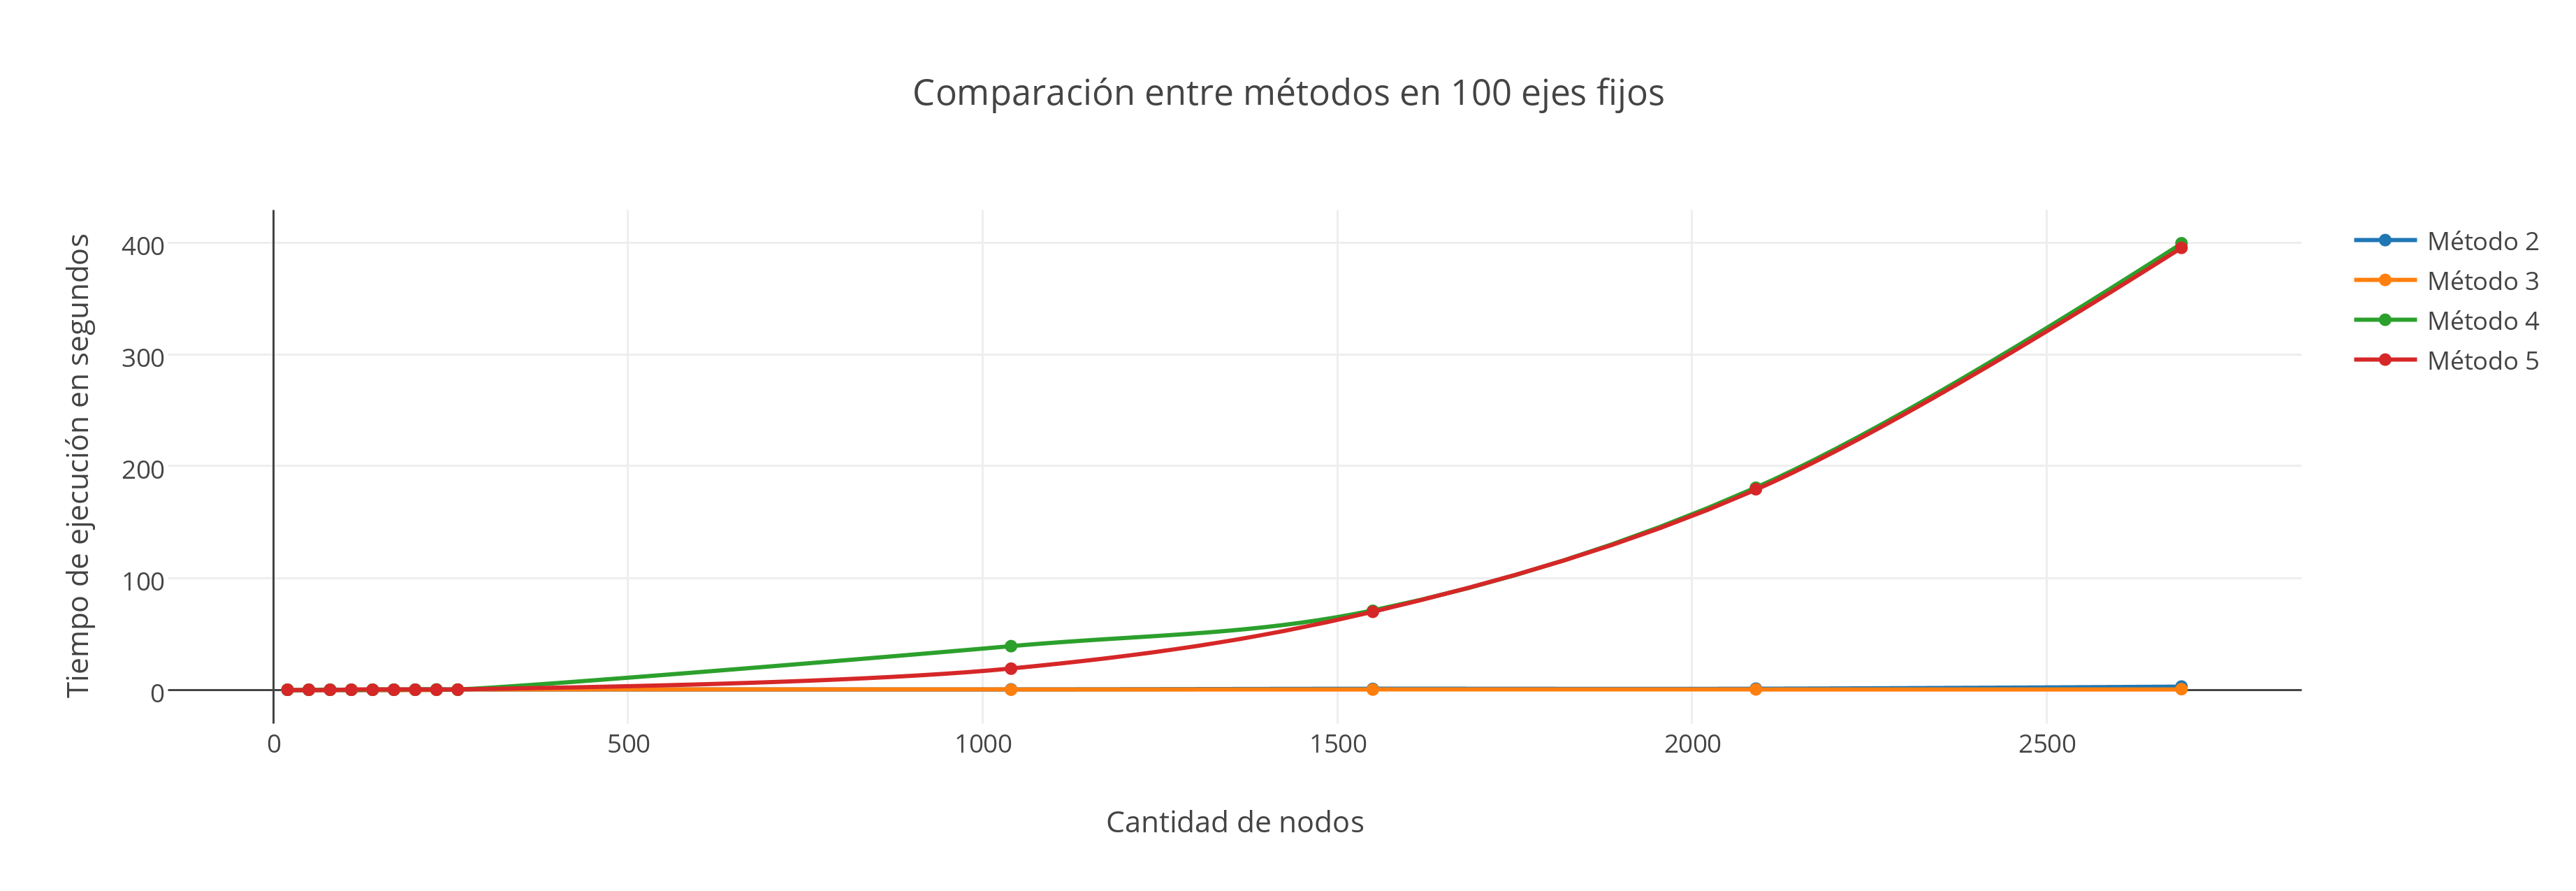
\includegraphics[scale=0.17]{imagenes/local/tiempos/100ejes.png}
% 	\caption{}
%	\label{10Nodos}
   \end{center}
 \end{figure}
 

  \begin{figure}[h!]
   \begin{center}
 	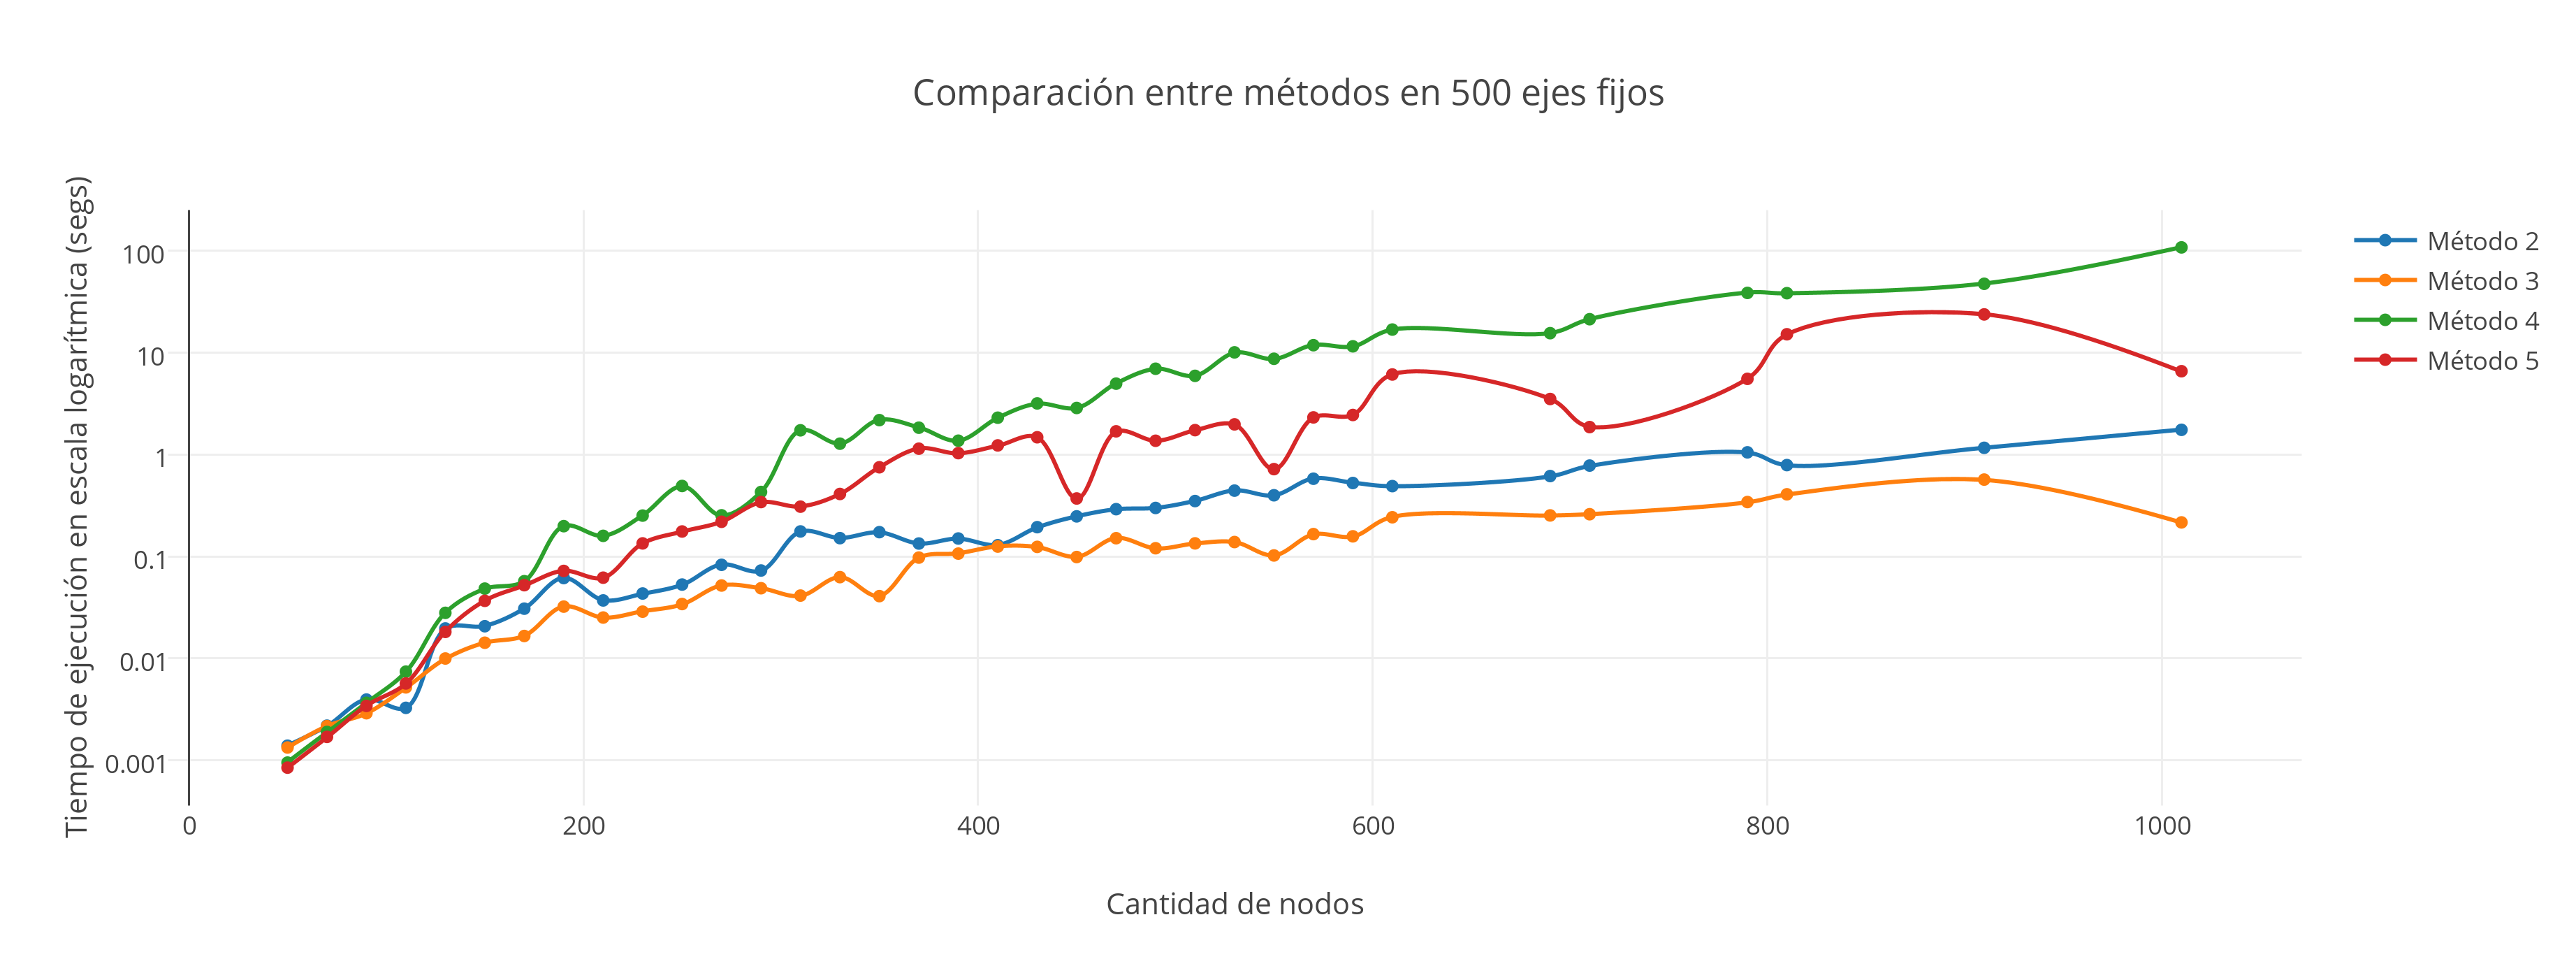
\includegraphics[scale=0.5]{imagenes/local/tiempos/500ejes.png}
% 	\caption{}
%	\label{10Nodos}
   \end{center}
 \end{figure}
 
   \begin{figure}[h!]
   \begin{center}
 	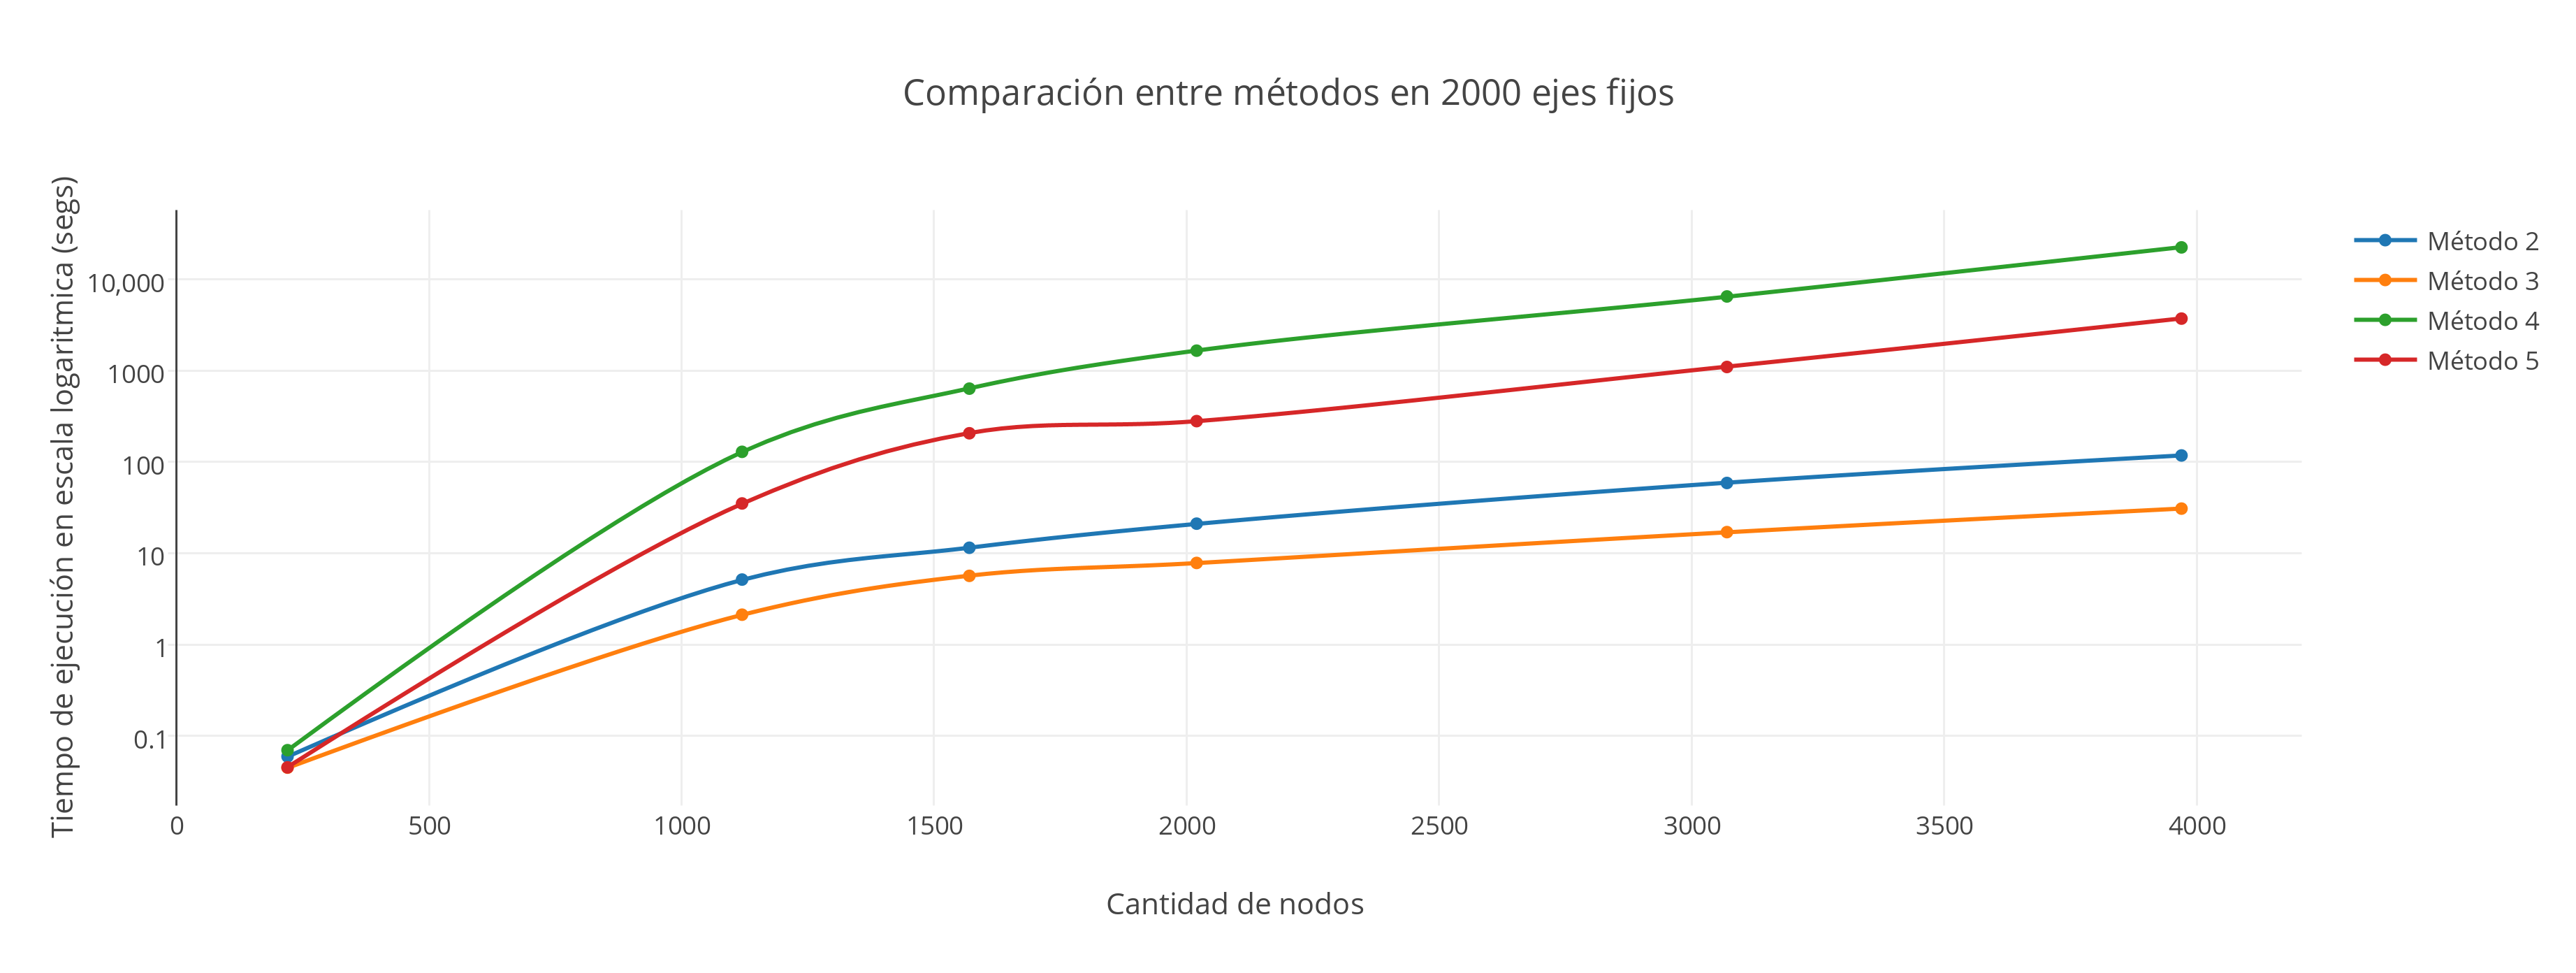
\includegraphics[scale=0.5]{imagenes/local/tiempos/2000ejes.png}
% 	\caption{}
%	\label{10Nodos}
   \end{center}
 \end{figure}
 
 \newpage
  \begin{figure}[h!]
   \begin{center}
 	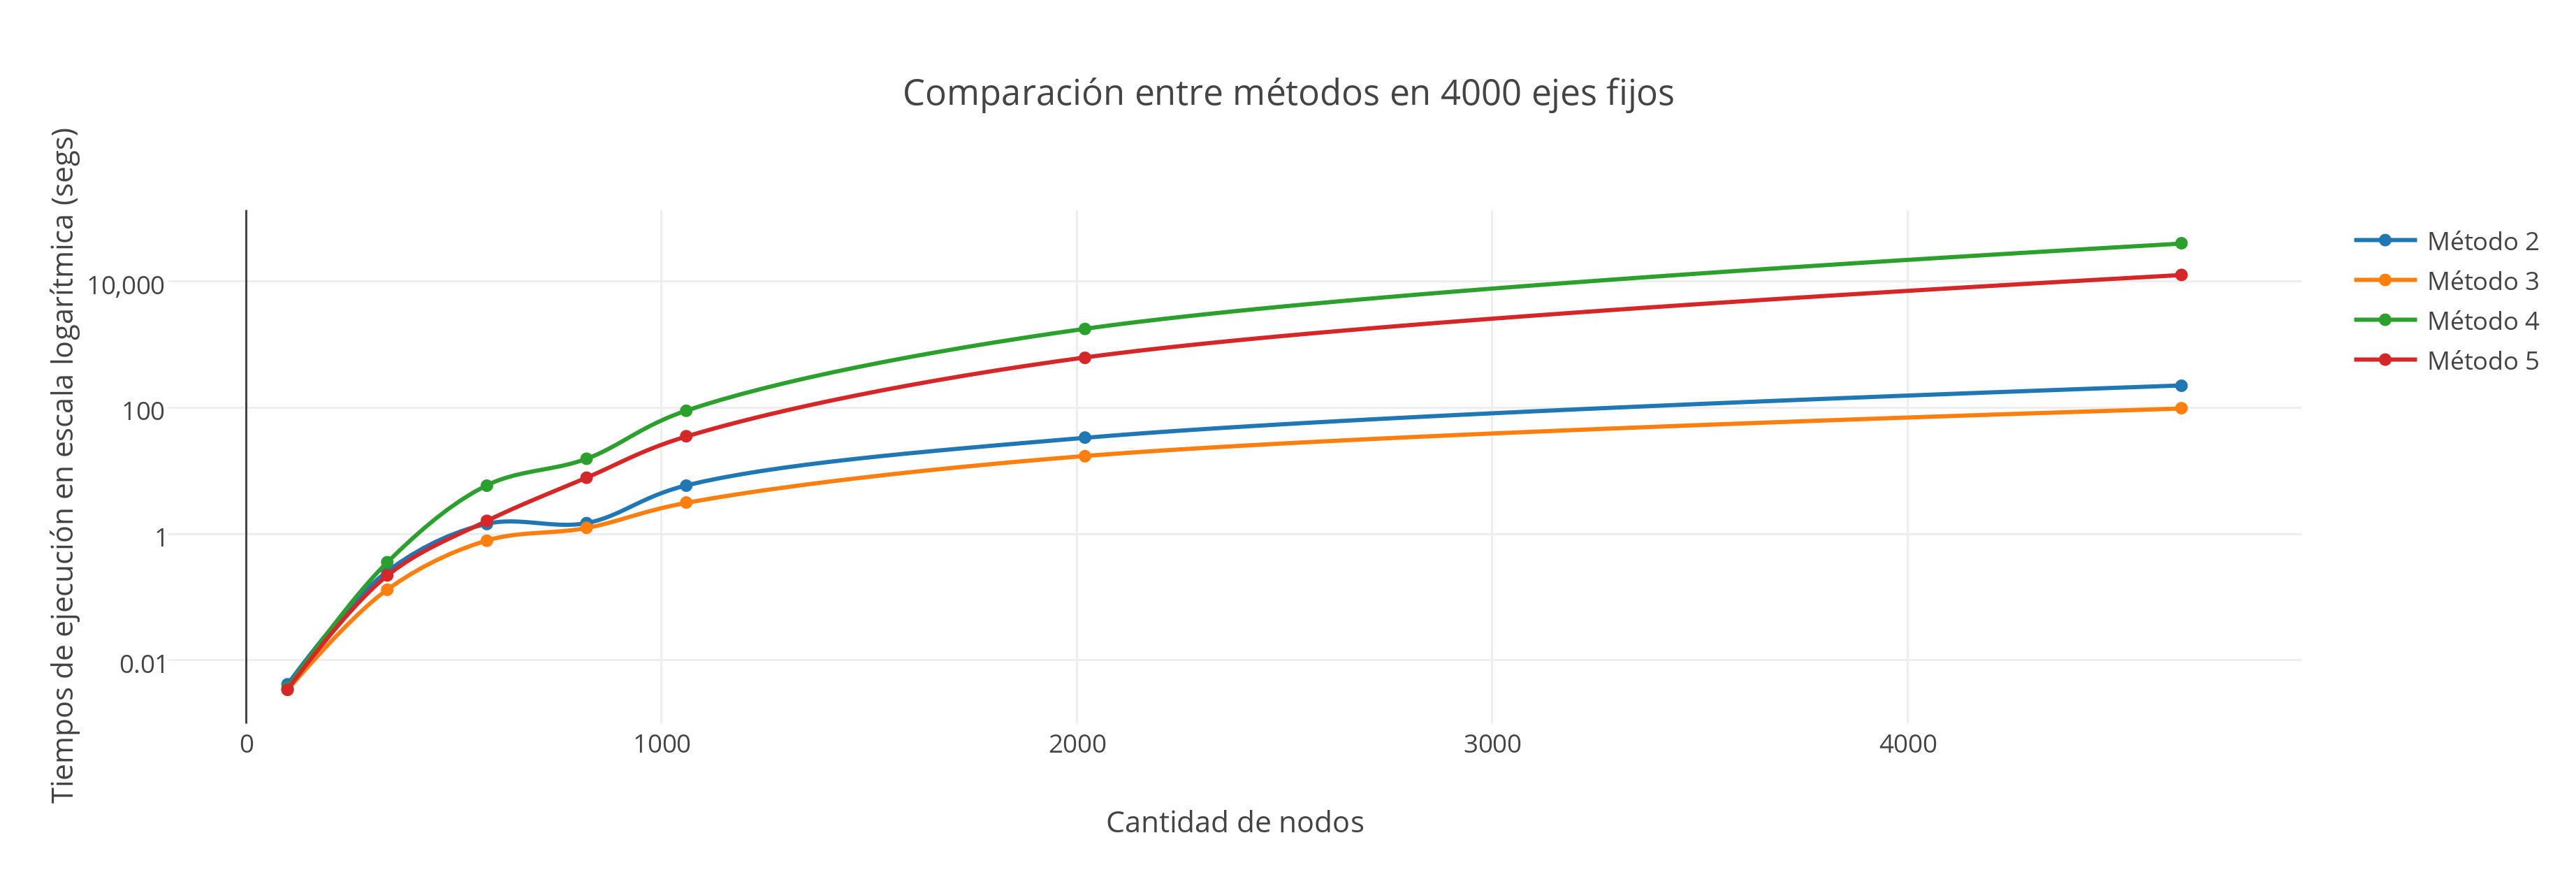
\includegraphics[scale=0.5]{imagenes/local/tiempos/4000ejes.png}
% 	\caption{}
%	\label{10Nodos}
   \end{center}
 \end{figure}
  
  \begin{figure}[h!]
   \begin{center}
 	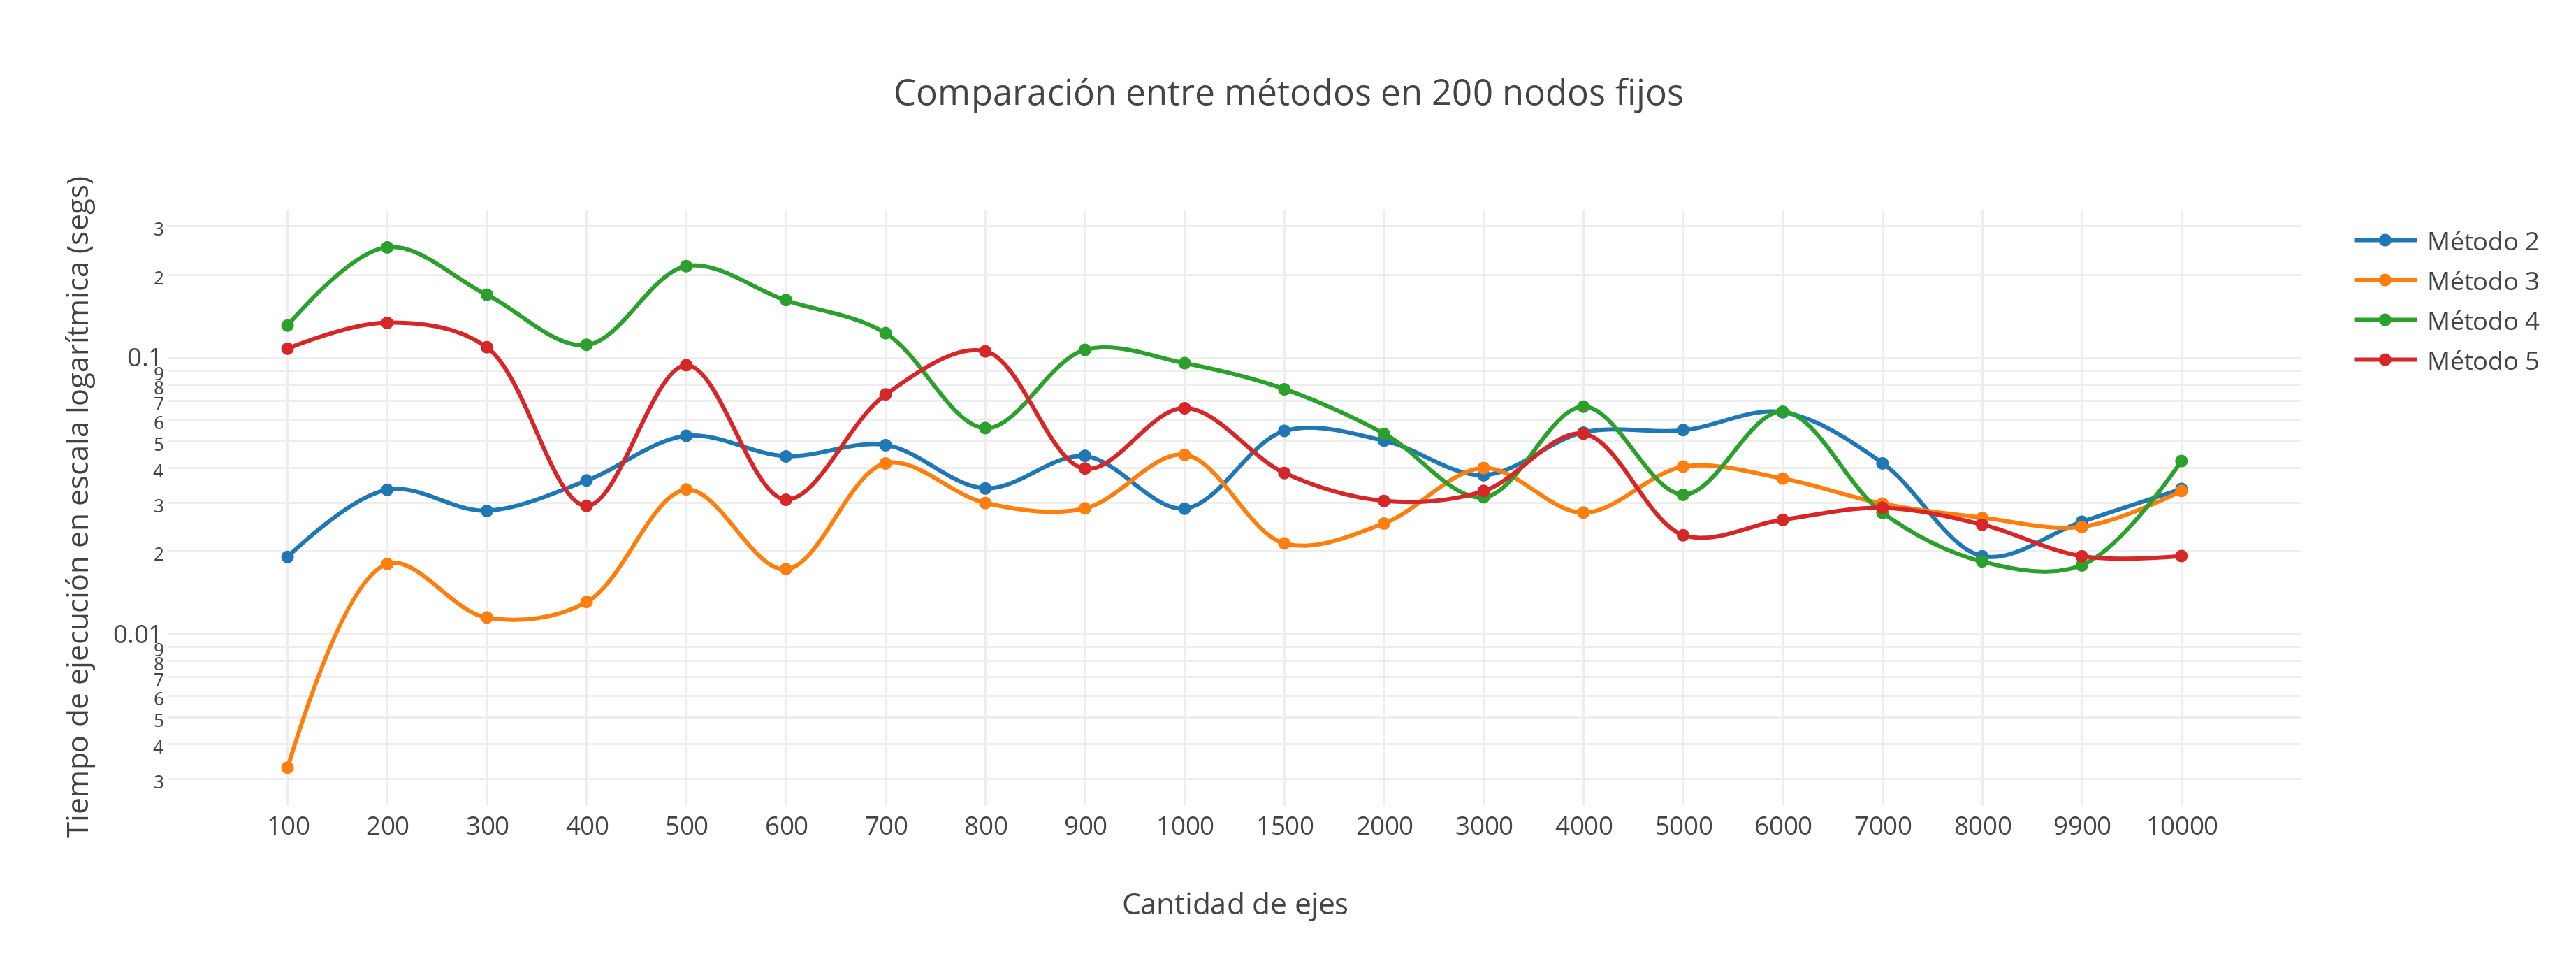
\includegraphics[scale=0.5]{imagenes/local/tiempos/200nodos.png}
% 	\caption{}
%	\label{10Nodos}
   \end{center}
 \end{figure}
 
  \begin{figure}[h!]
   \begin{center}
 	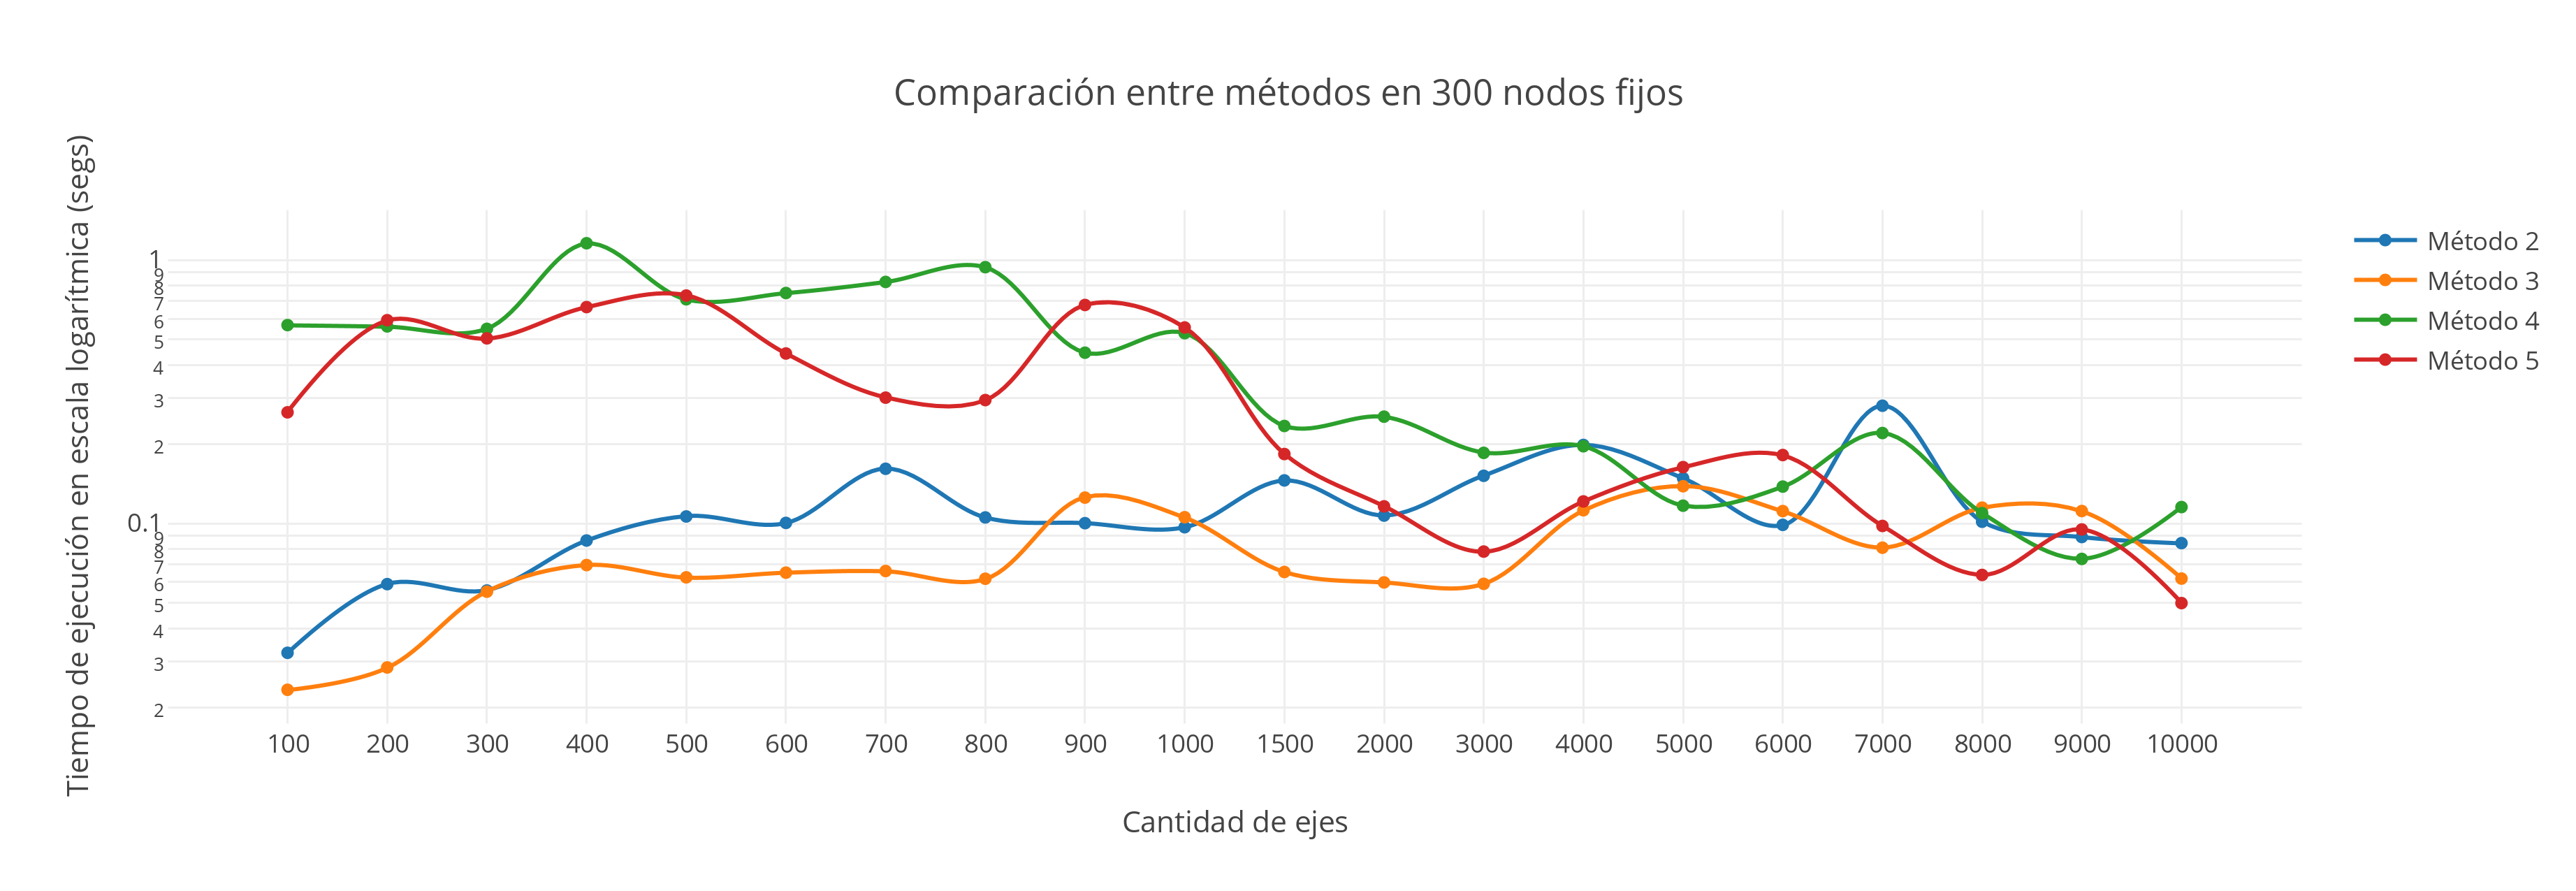
\includegraphics[scale=0.5]{imagenes/local/tiempos/300nodos.png}
% 	\caption{}
%	\label{10Nodos}
   \end{center}
 \end{figure}
 
 \newpage
  \begin{figure}[h!]
   \begin{center}
 	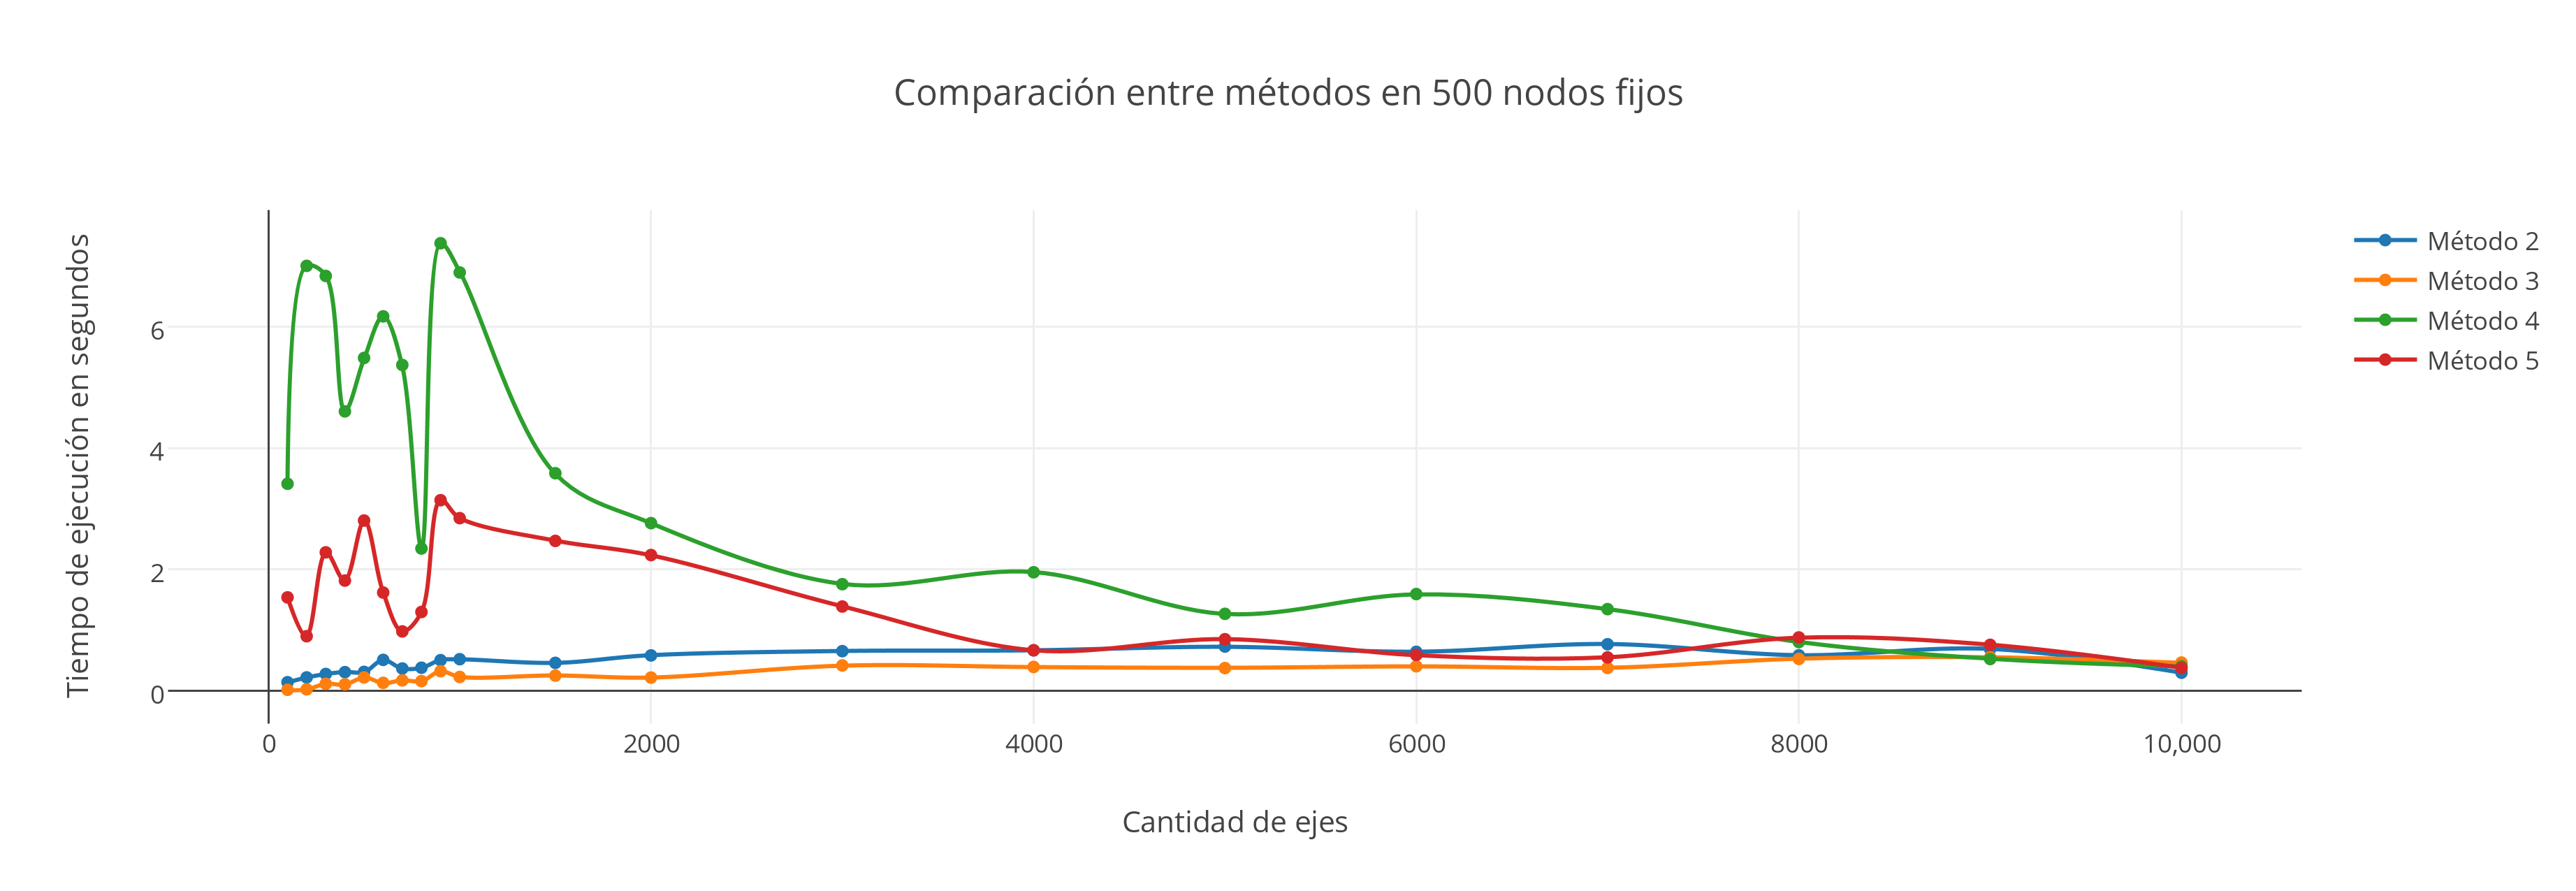
\includegraphics[scale=0.5]{imagenes/local/tiempos/500nodos.png}
% 	\caption{}
%	\label{10Nodos}
   \end{center}
 \end{figure}
 
   \begin{figure}[h!]
   \begin{center}
 	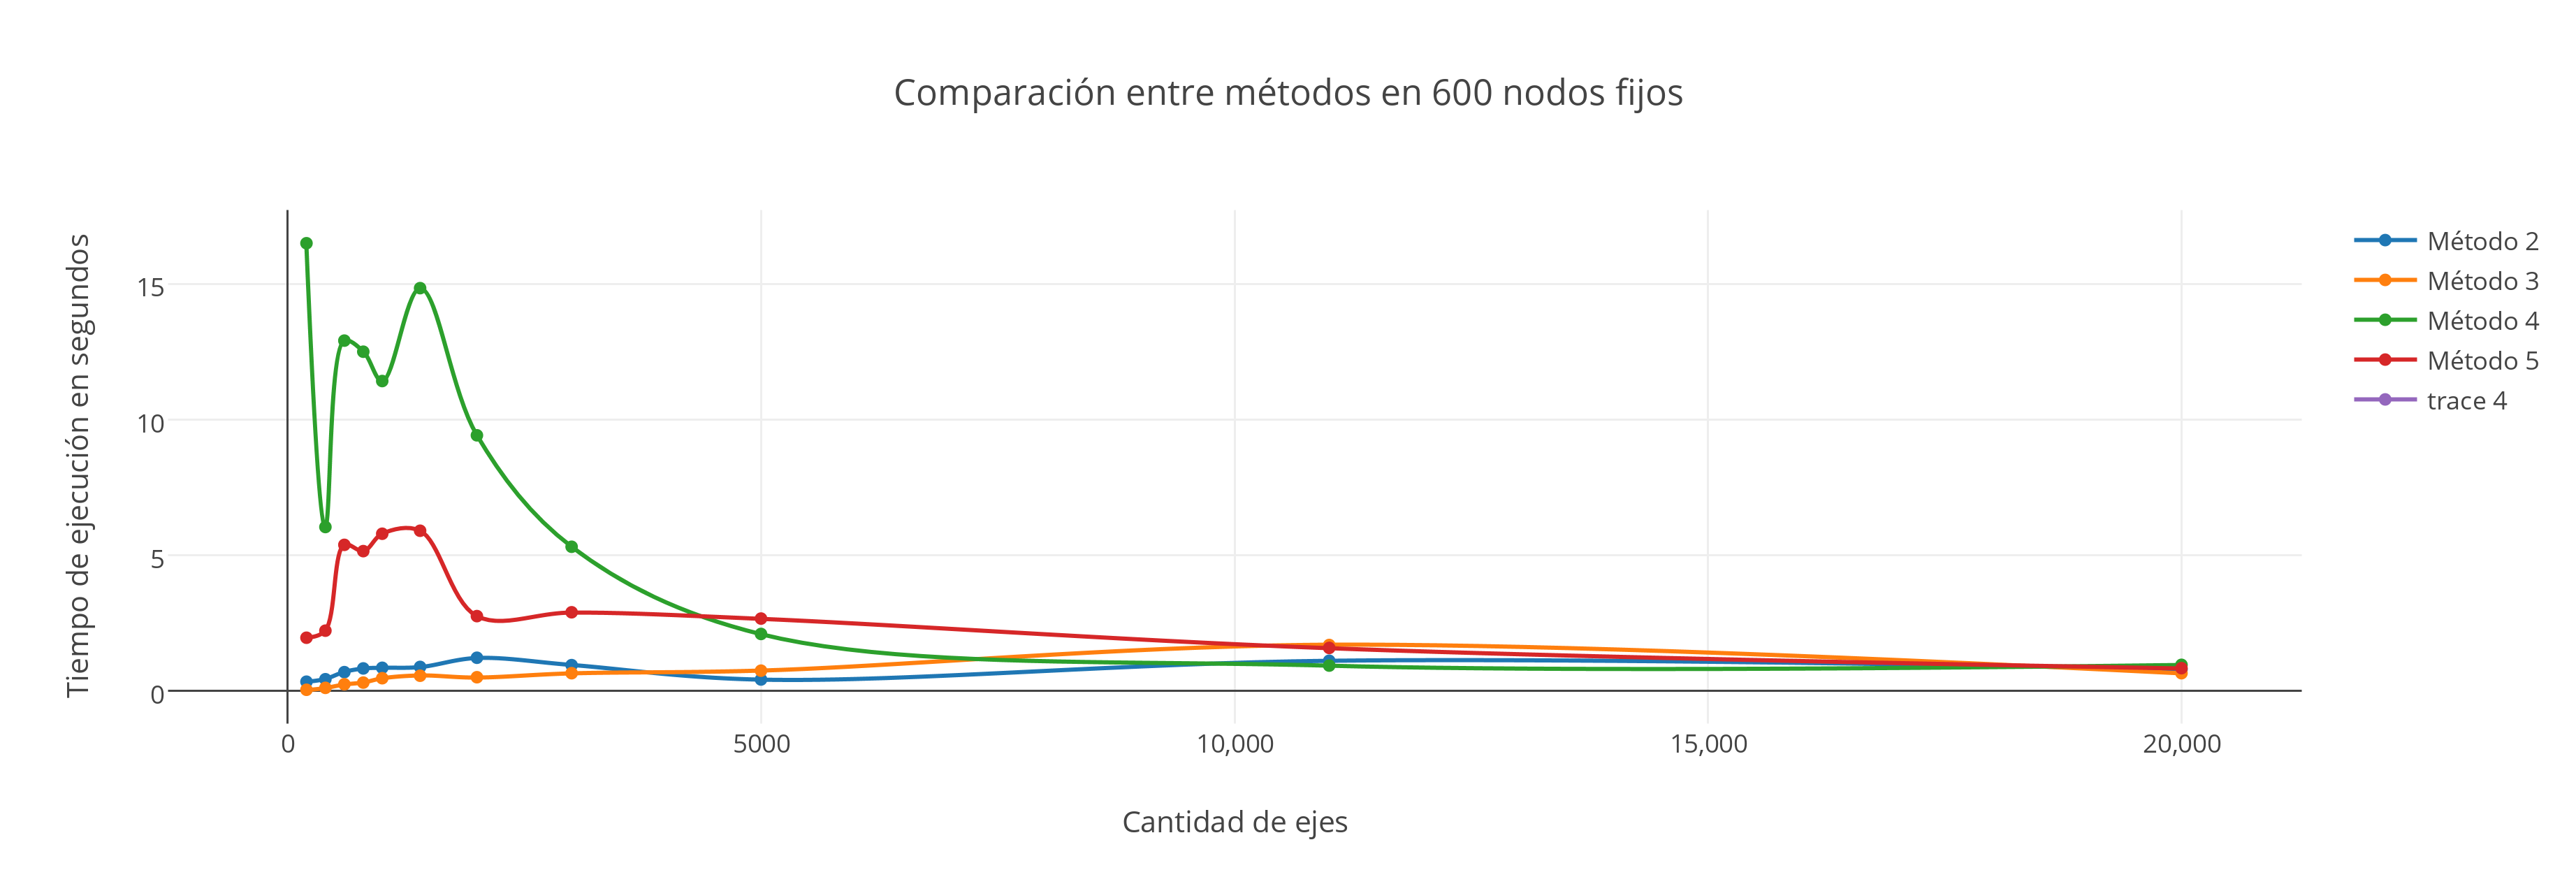
\includegraphics[scale=0.5]{imagenes/local/tiempos/600nodos.png}
% 	\caption{}
%	\label{10Nodos}
   \end{center}
 \end{figure}

  \begin{figure}[h!]
   \begin{center}
 	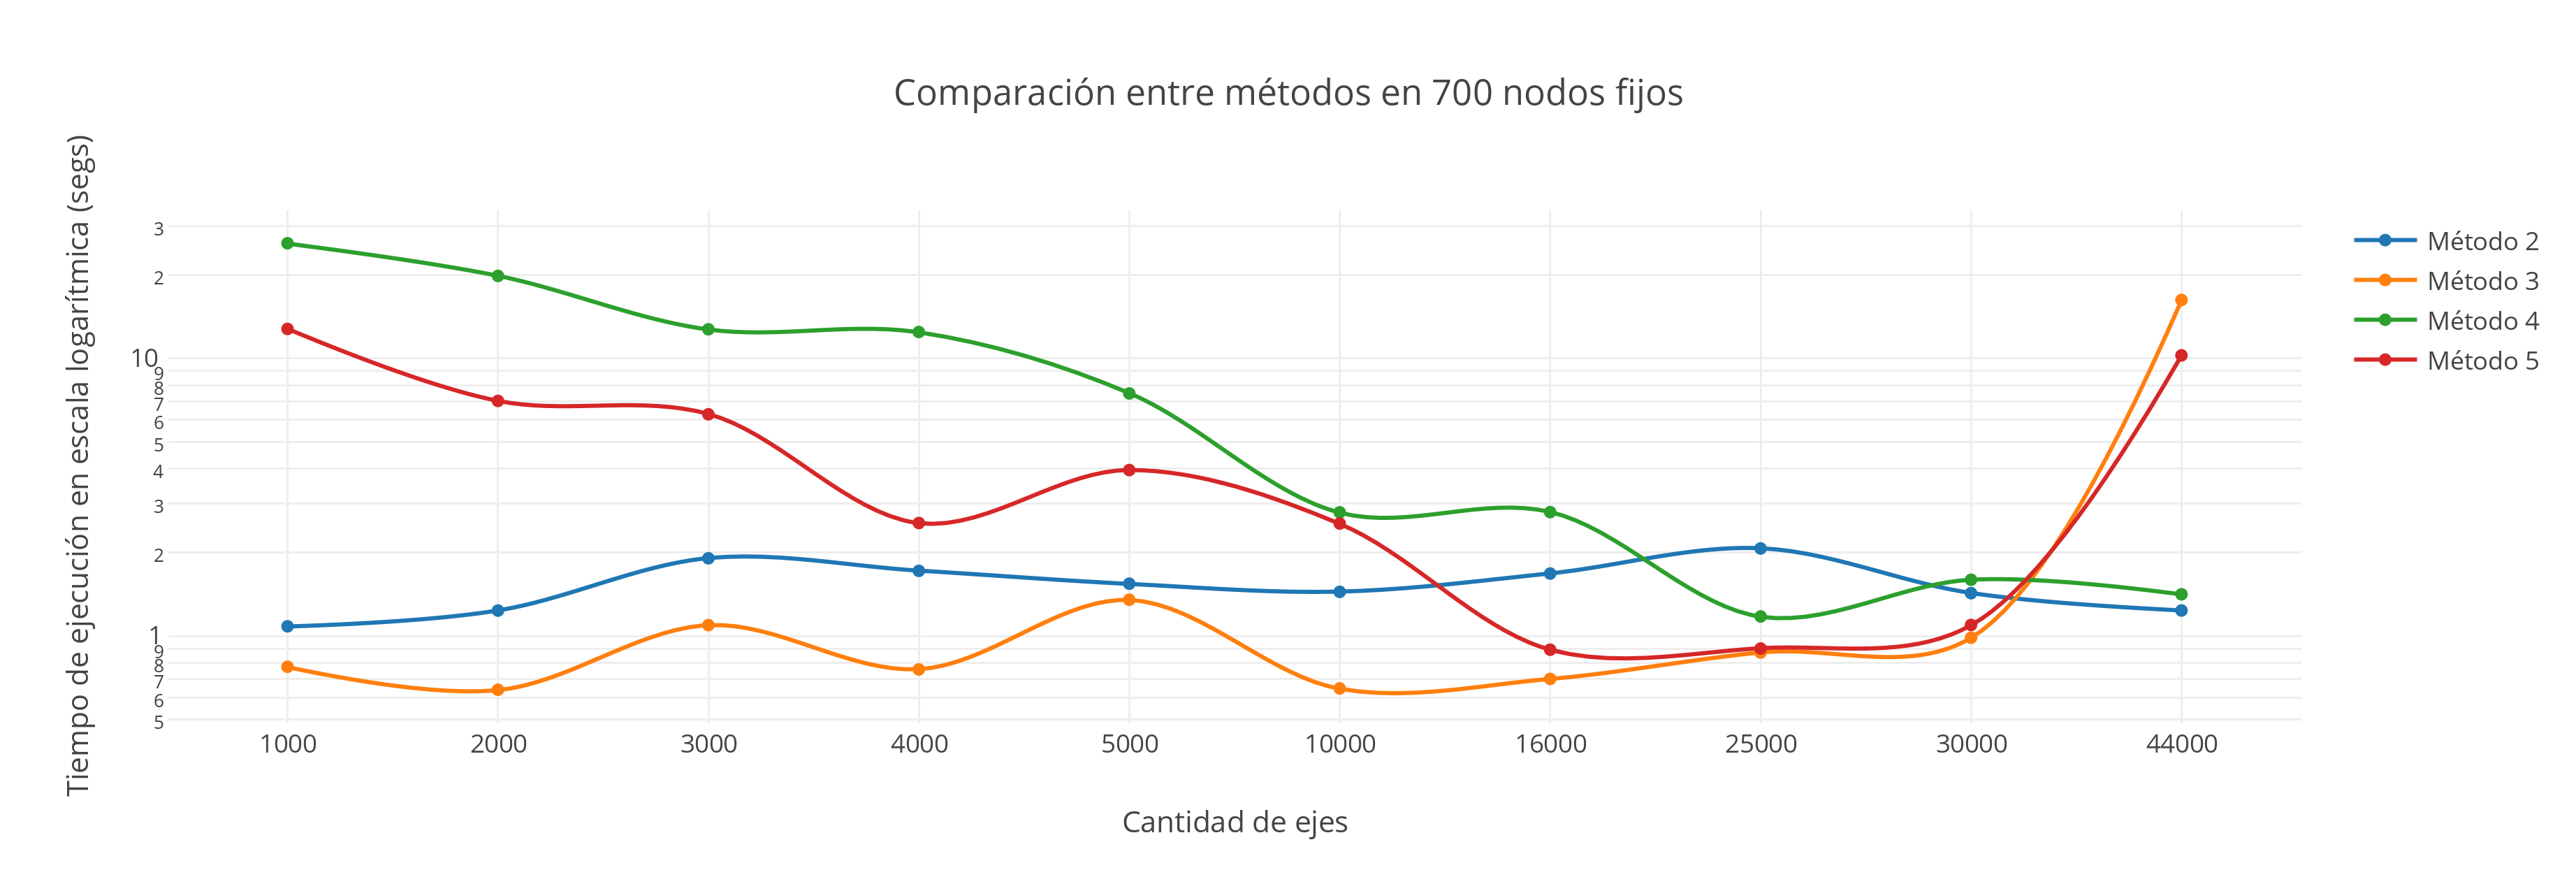
\includegraphics[scale=0.5]{imagenes/local/tiempos/700nodos.png}
% 	\caption{}
%	\label{10Nodos}
   \end{center}
 \end{figure} 
 
\subsubsection{Contrastaci\'on emp\'irica de la complejidad}

\newpage
\subsubsection{Comparaci\'on soluciones Local vs Exacto}

  \begin{figure}[h!]
   \begin{center}
 	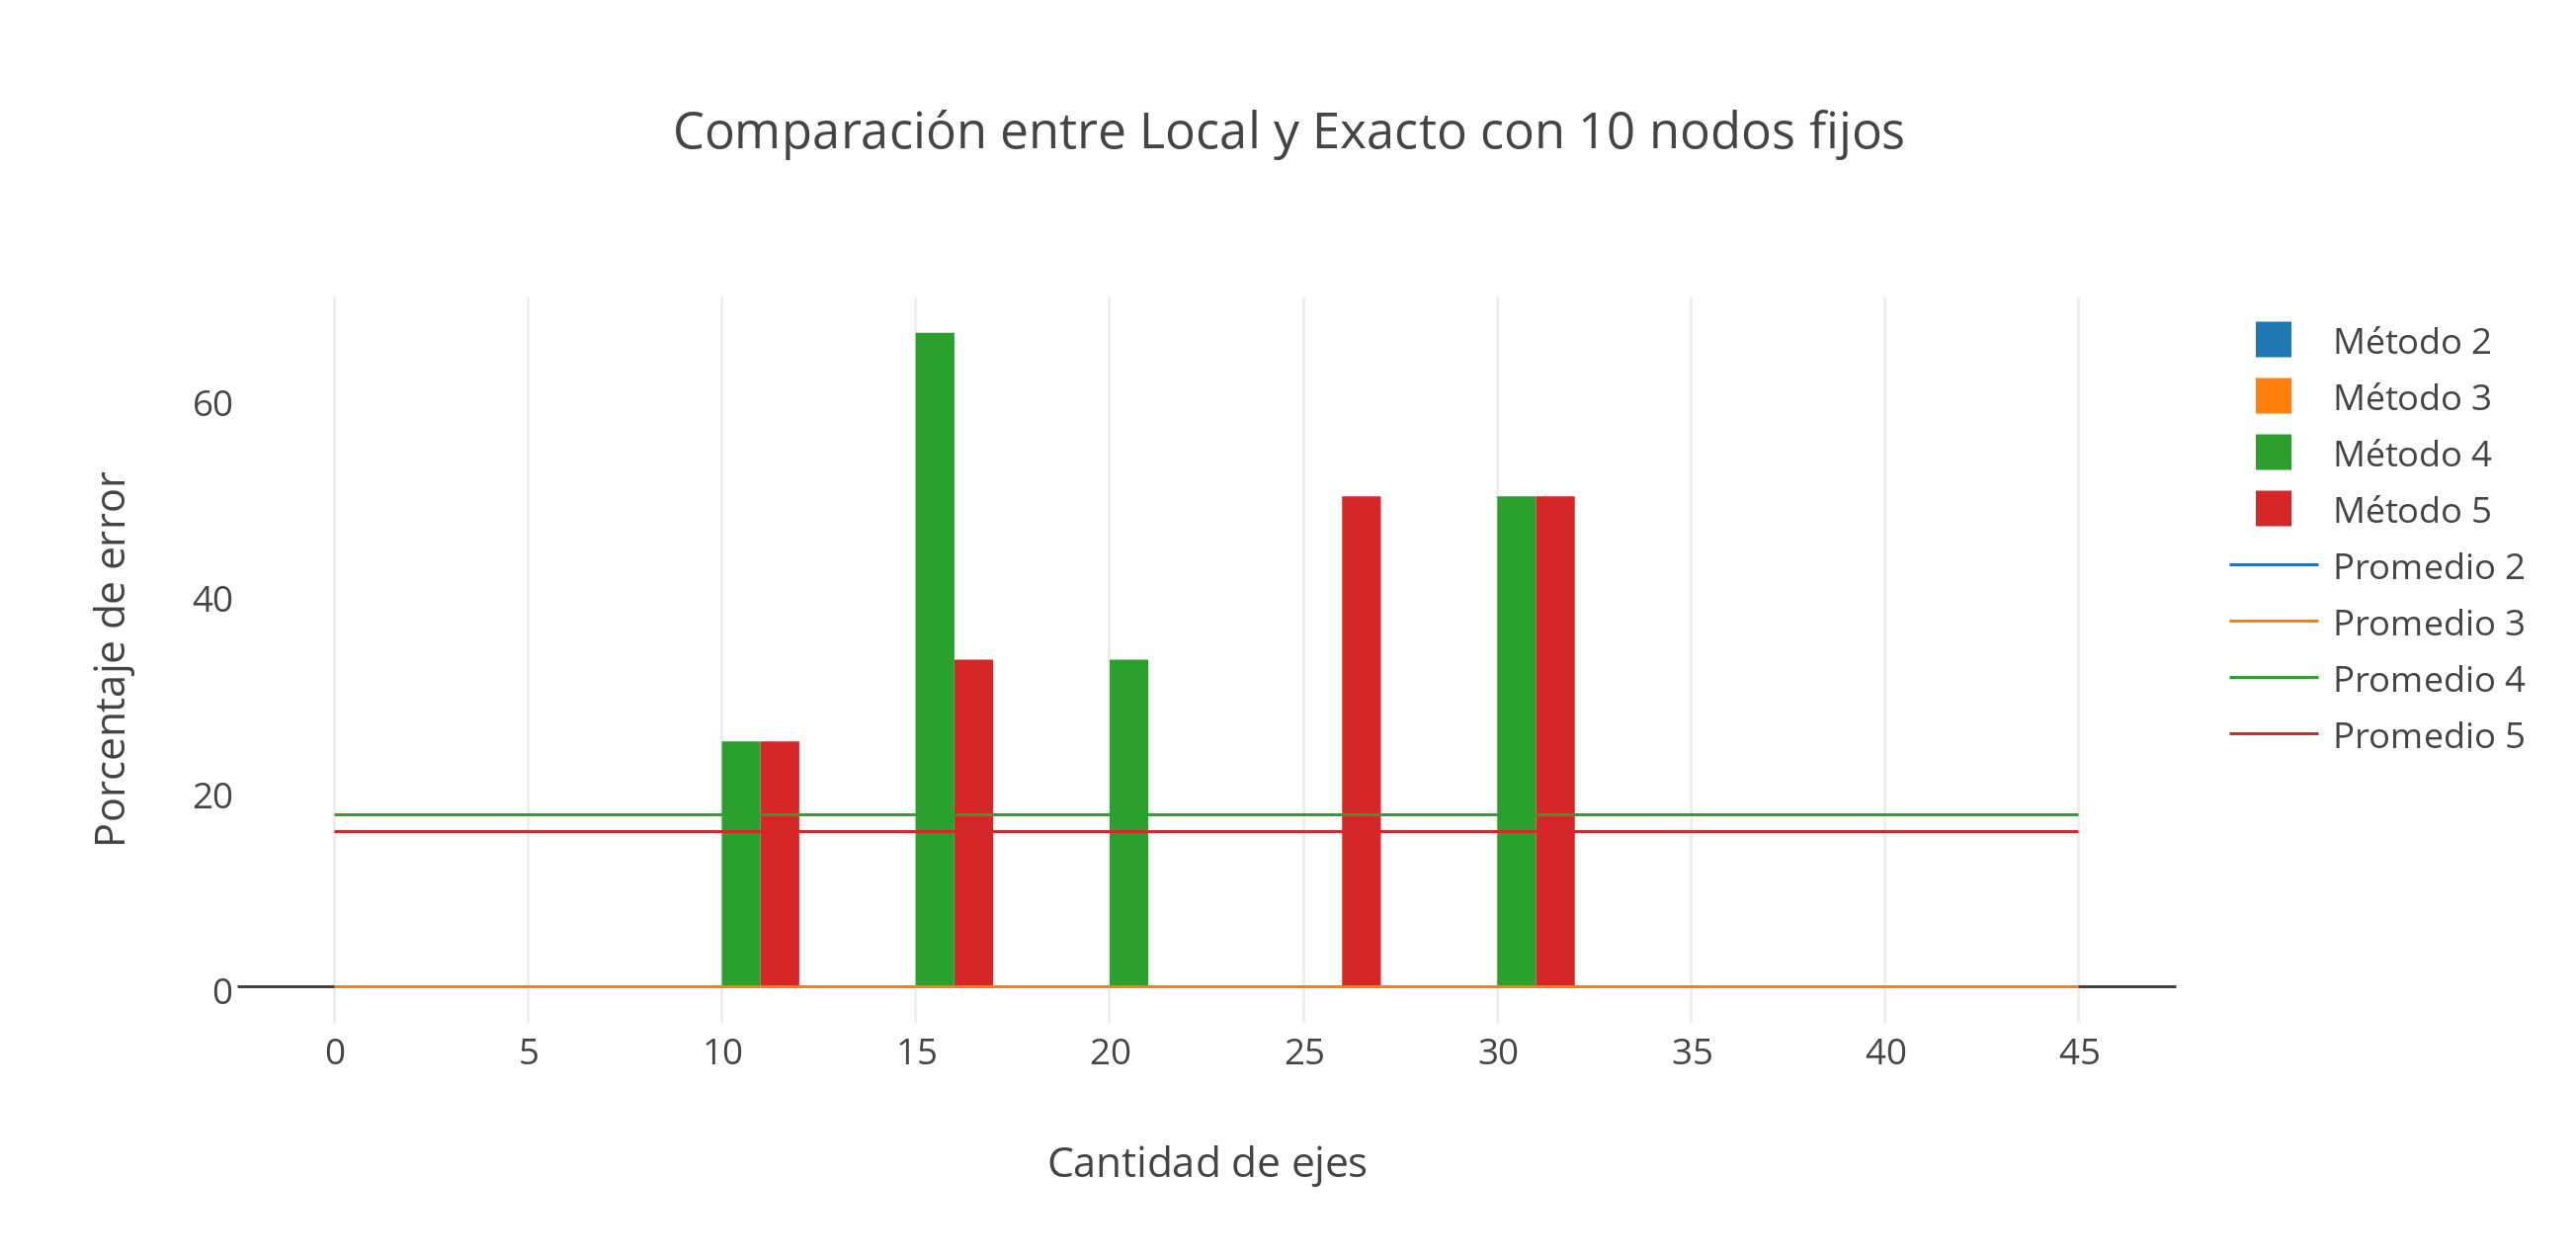
\includegraphics[scale=0.75]{imagenes/local/exacto/10nodos.png}
% 	\caption{}
%	\label{10Nodos}
   \end{center}
 \end{figure}

  \begin{figure}[h!]
   \begin{center}
 	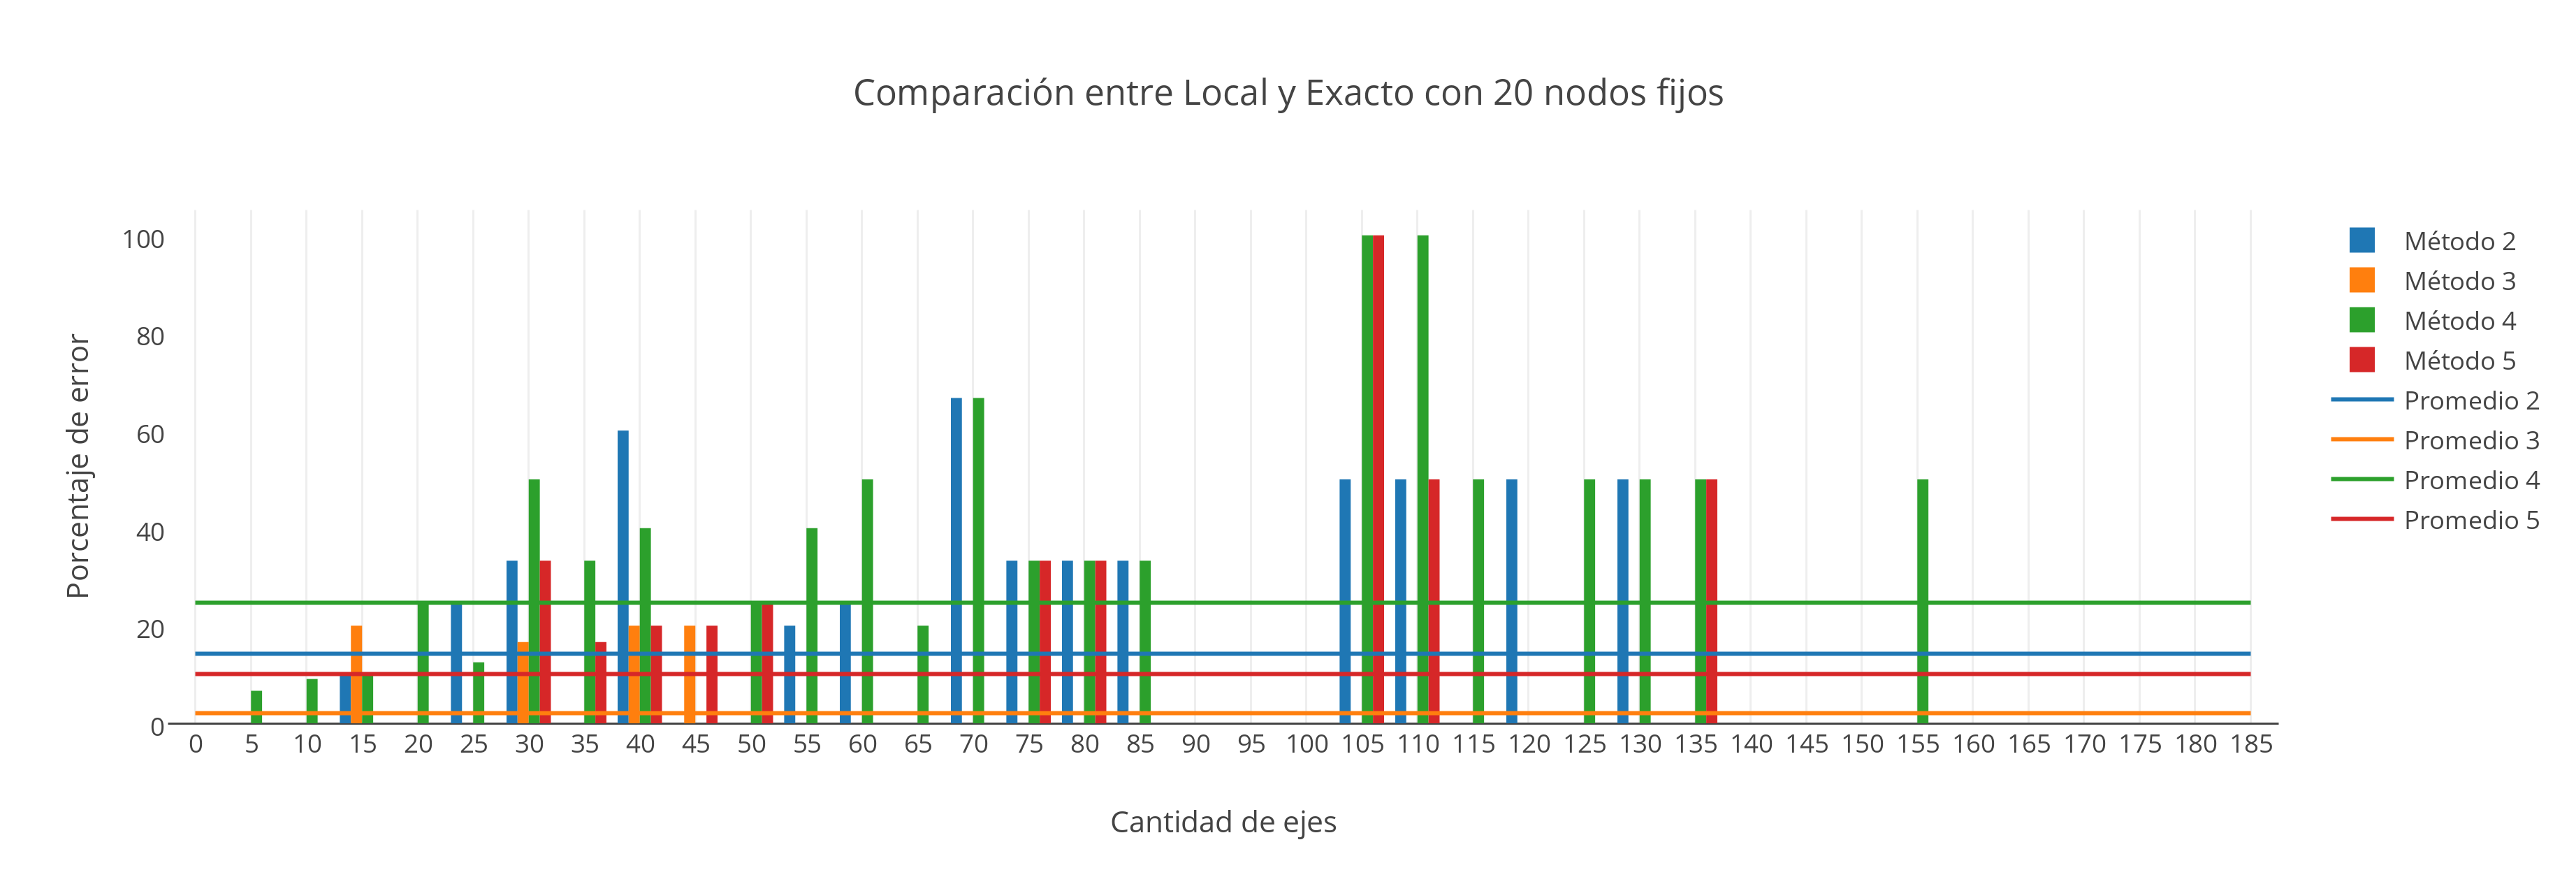
\includegraphics[scale=0.55]{imagenes/local/exacto/20nodos.png}
% 	\caption{}
%	\label{10Nodos}
   \end{center}
 \end{figure}
 
   \begin{figure}[h!]
   \begin{center}
 	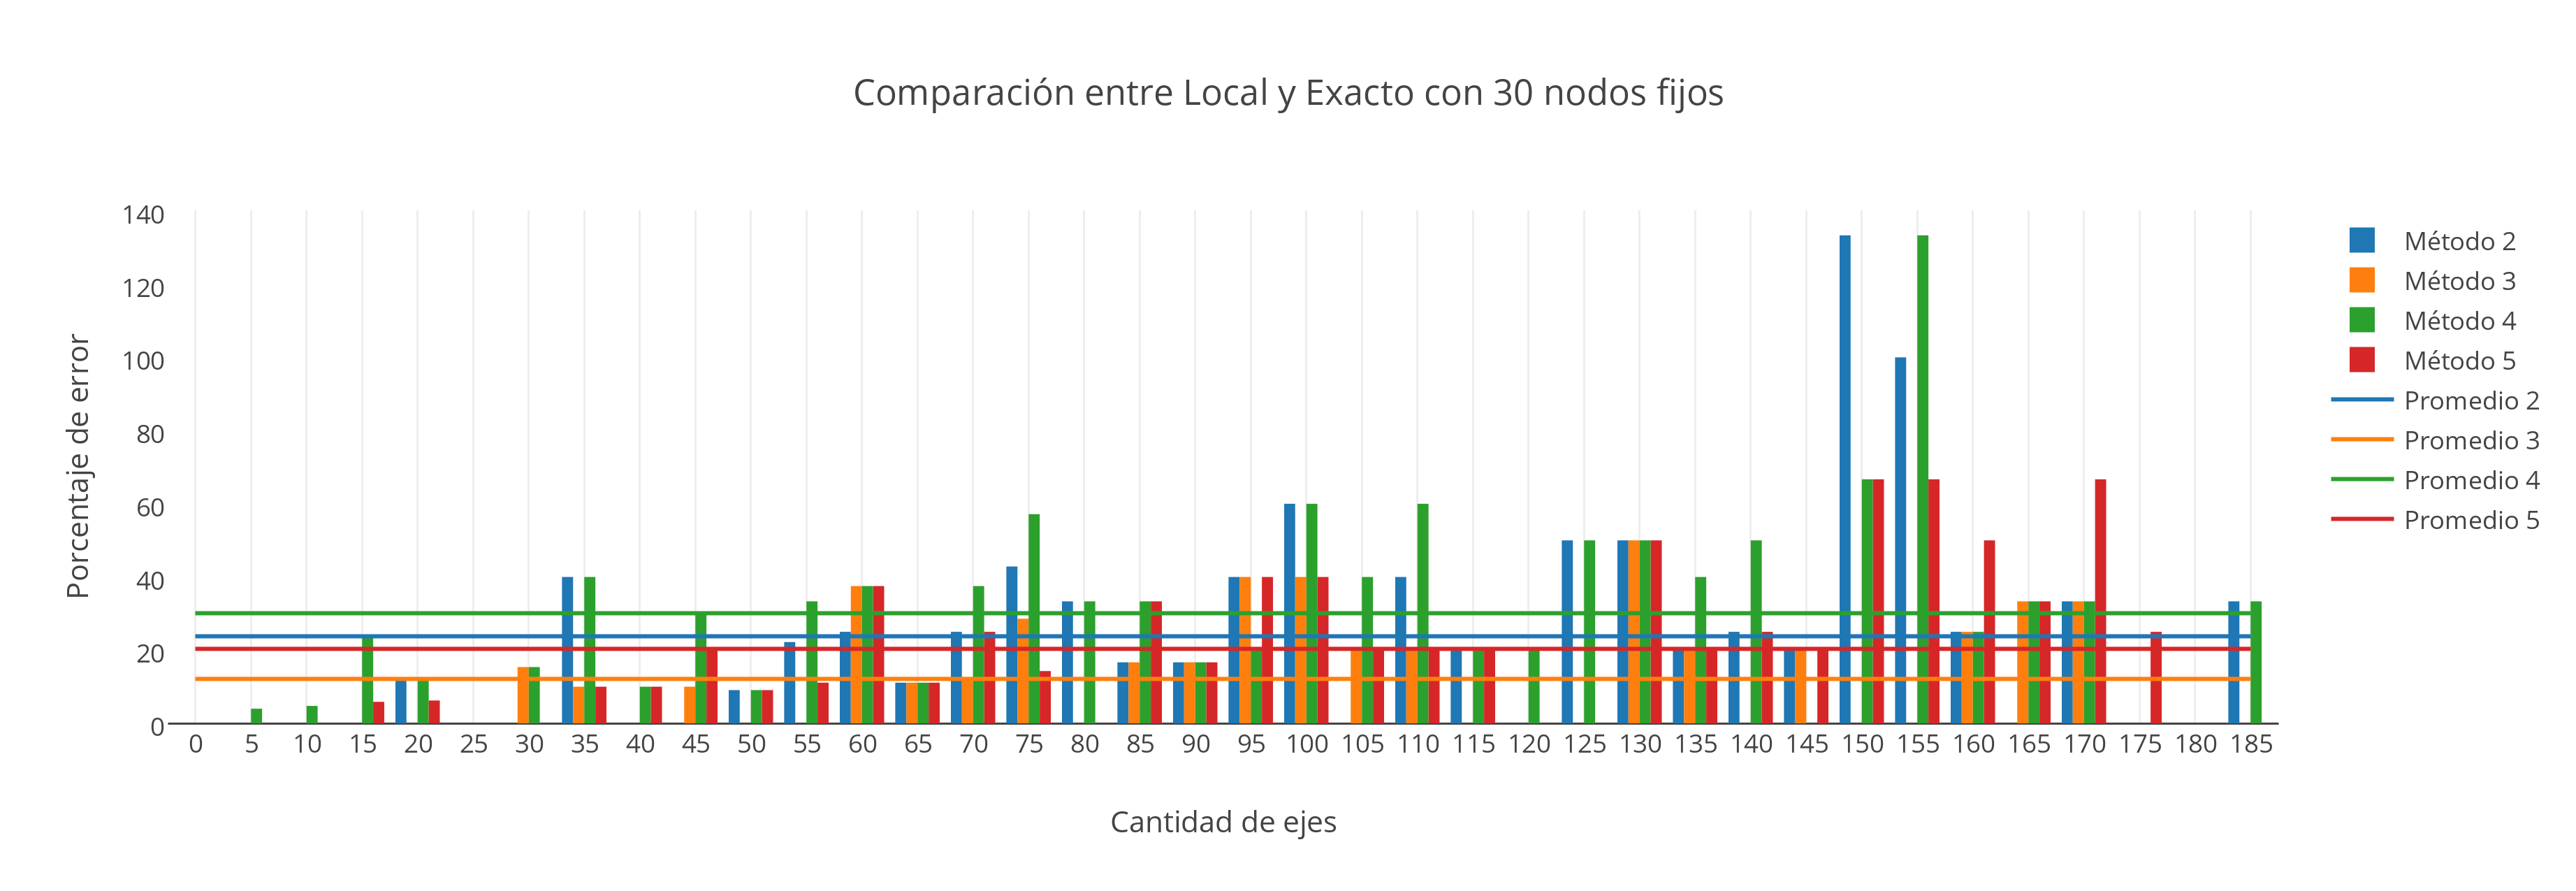
\includegraphics[scale=0.55]{imagenes/local/exacto/30nodos.png}
% 	\caption{}
%	\label{10Nodos}
   \end{center}
 \end{figure}

\newpage

  \begin{figure}[h!]
   \begin{center}
 	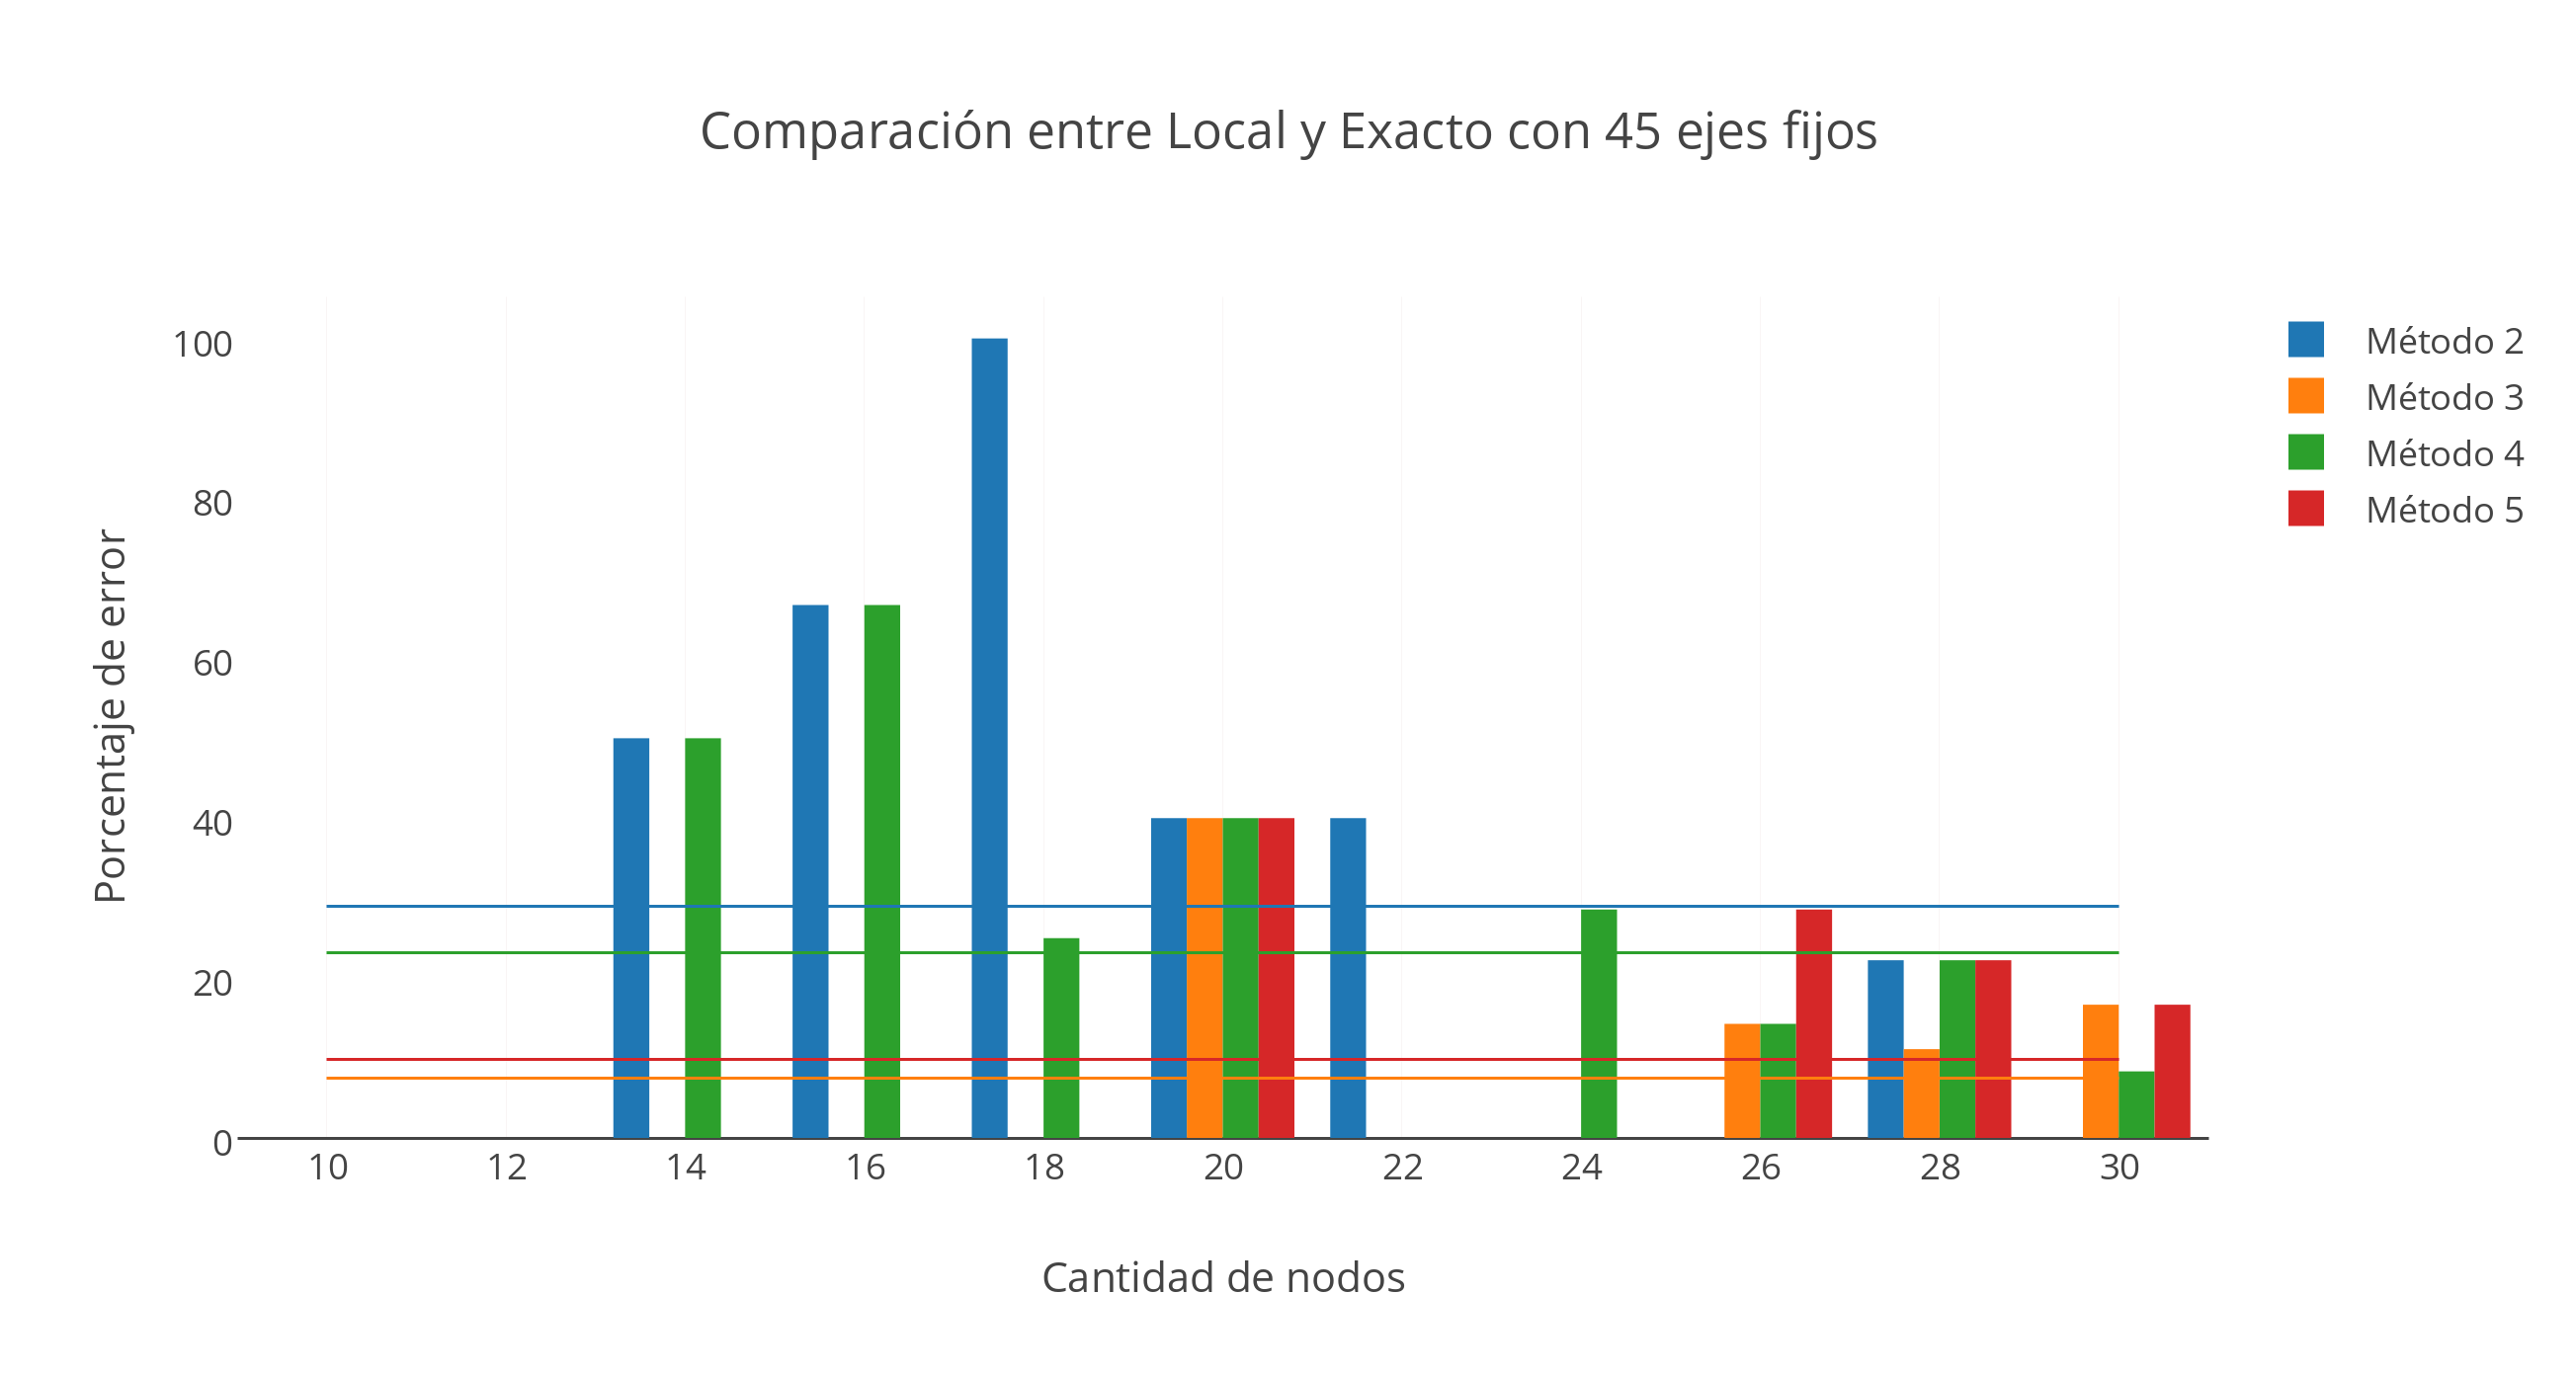
\includegraphics[scale=0.7]{imagenes/local/exacto/45ejes.png}
% 	\caption{}
%	\label{10Nodos}
   \end{center}
 \end{figure} 
 
  \begin{figure}[h!]
   \begin{center}
 	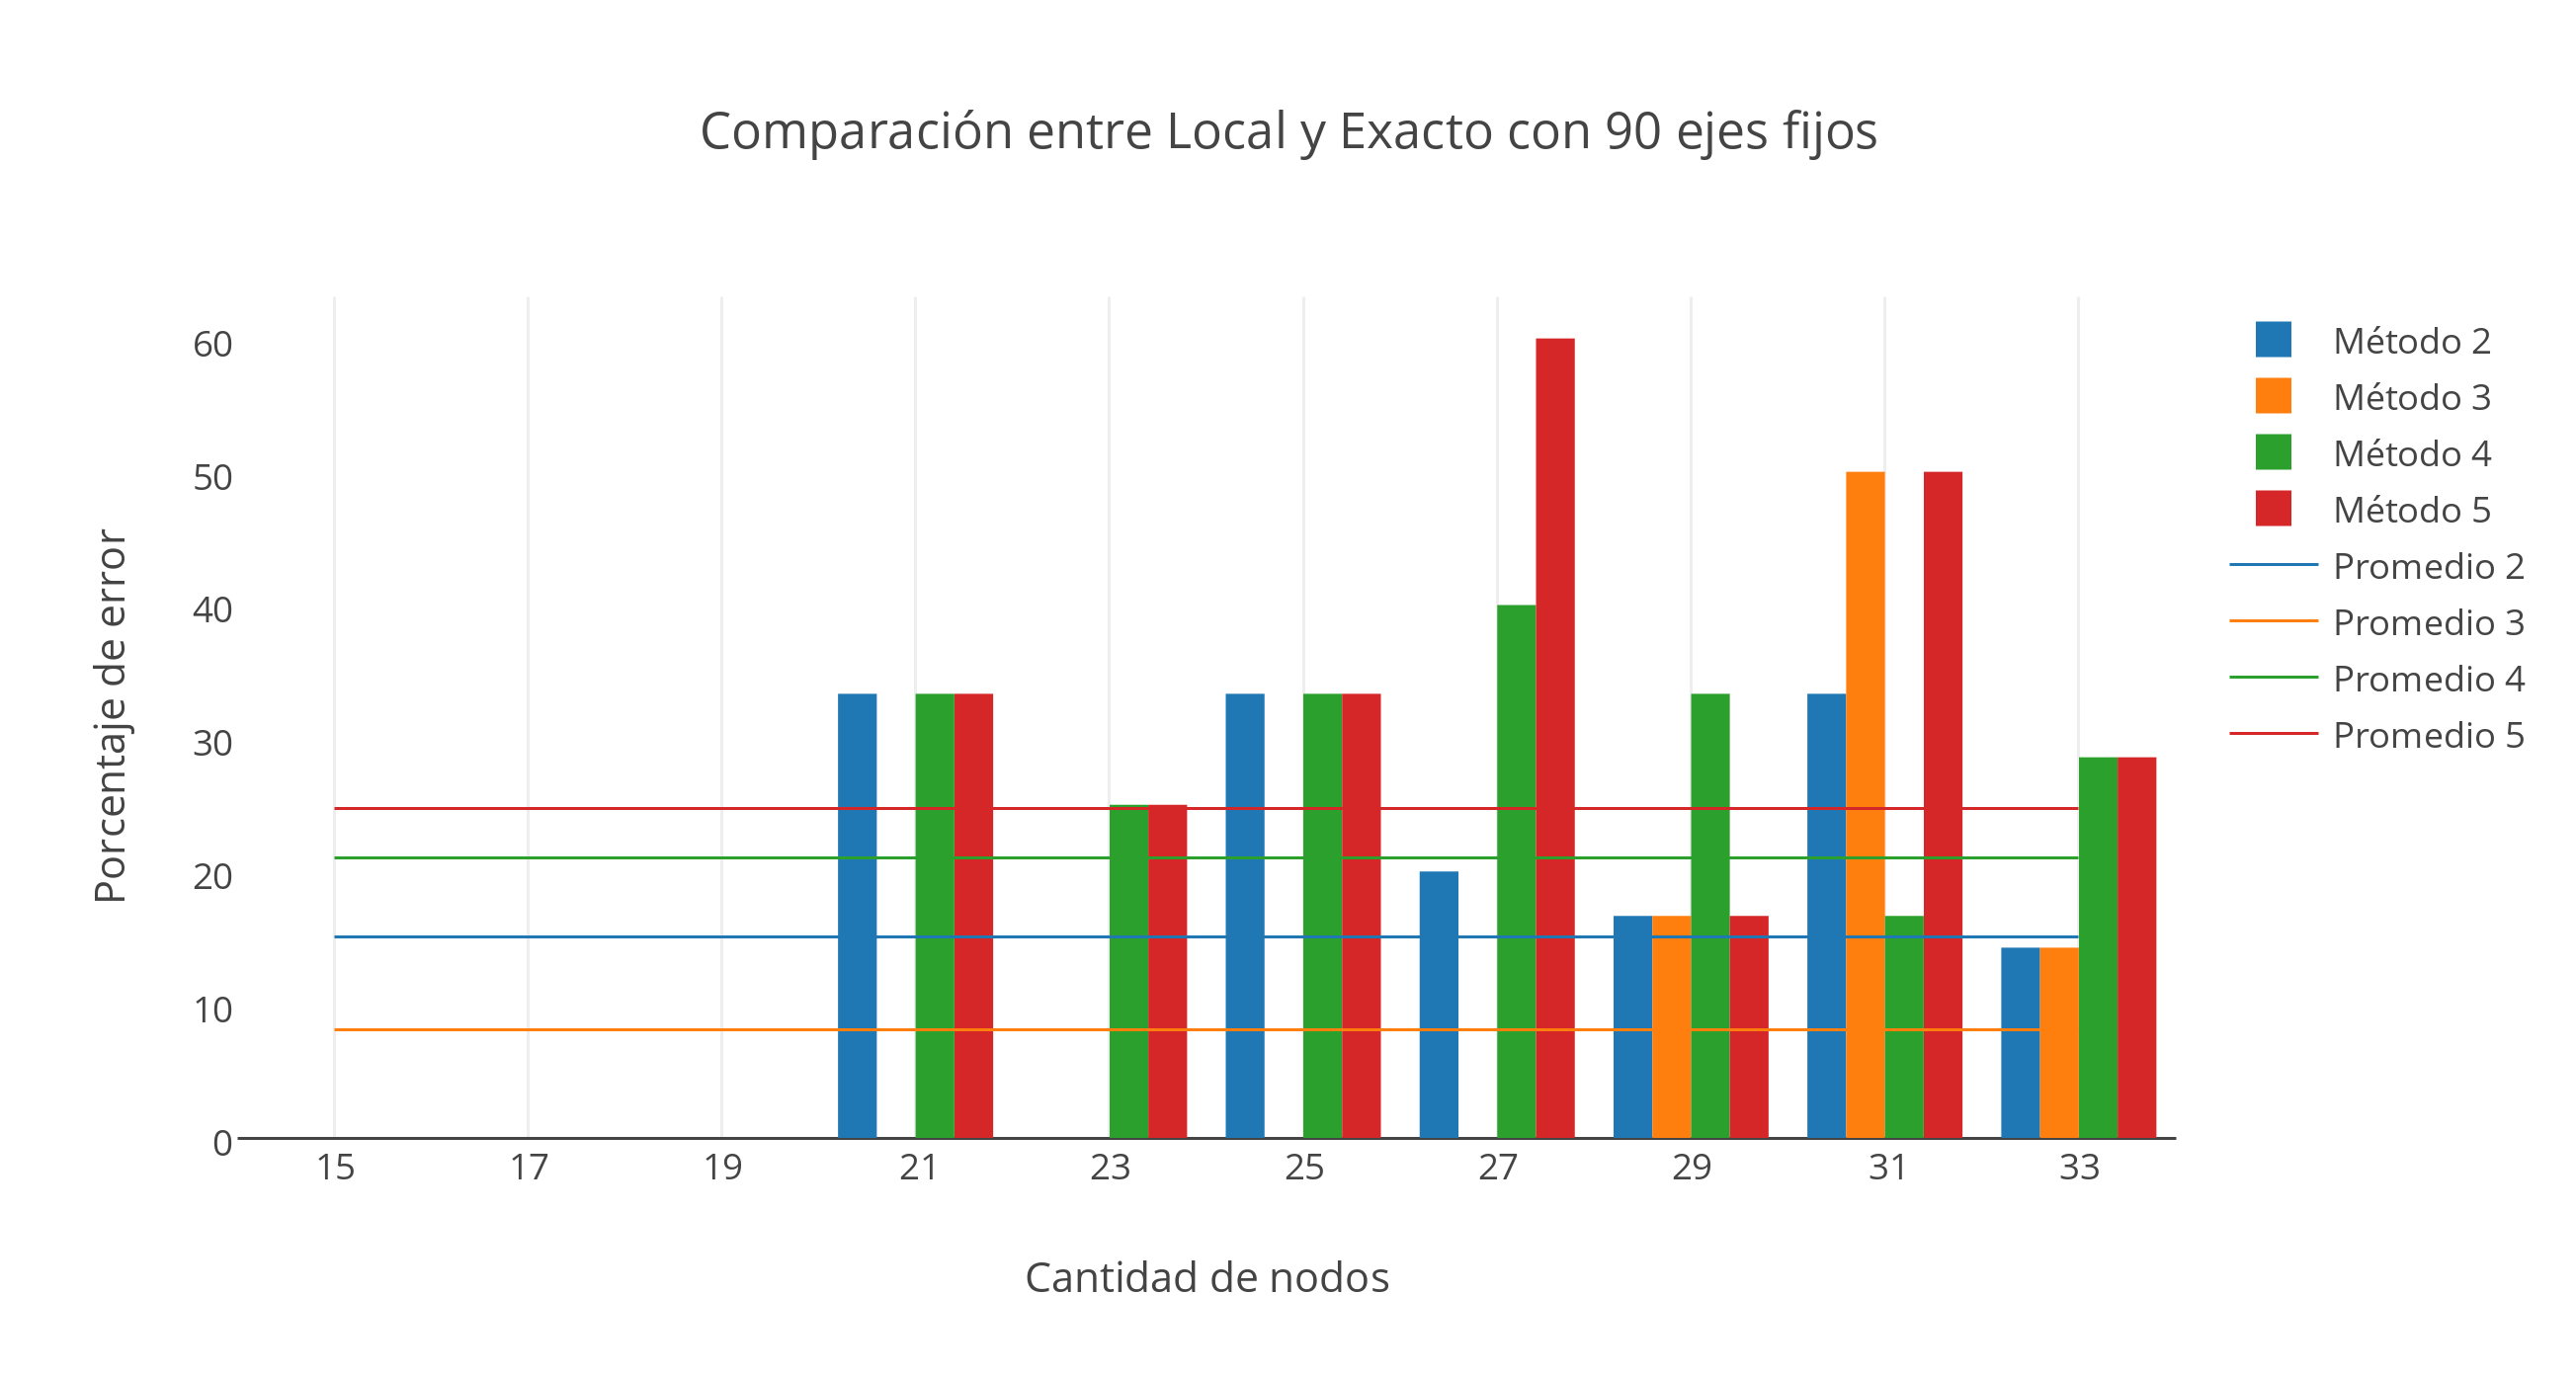
\includegraphics[scale=0.7]{imagenes/local/exacto/90ejes.png}
% 	\caption{}
%	\label{10Nodos}
   \end{center}
 \end{figure} 
 
  \begin{figure}[h!]
   \begin{center}
 	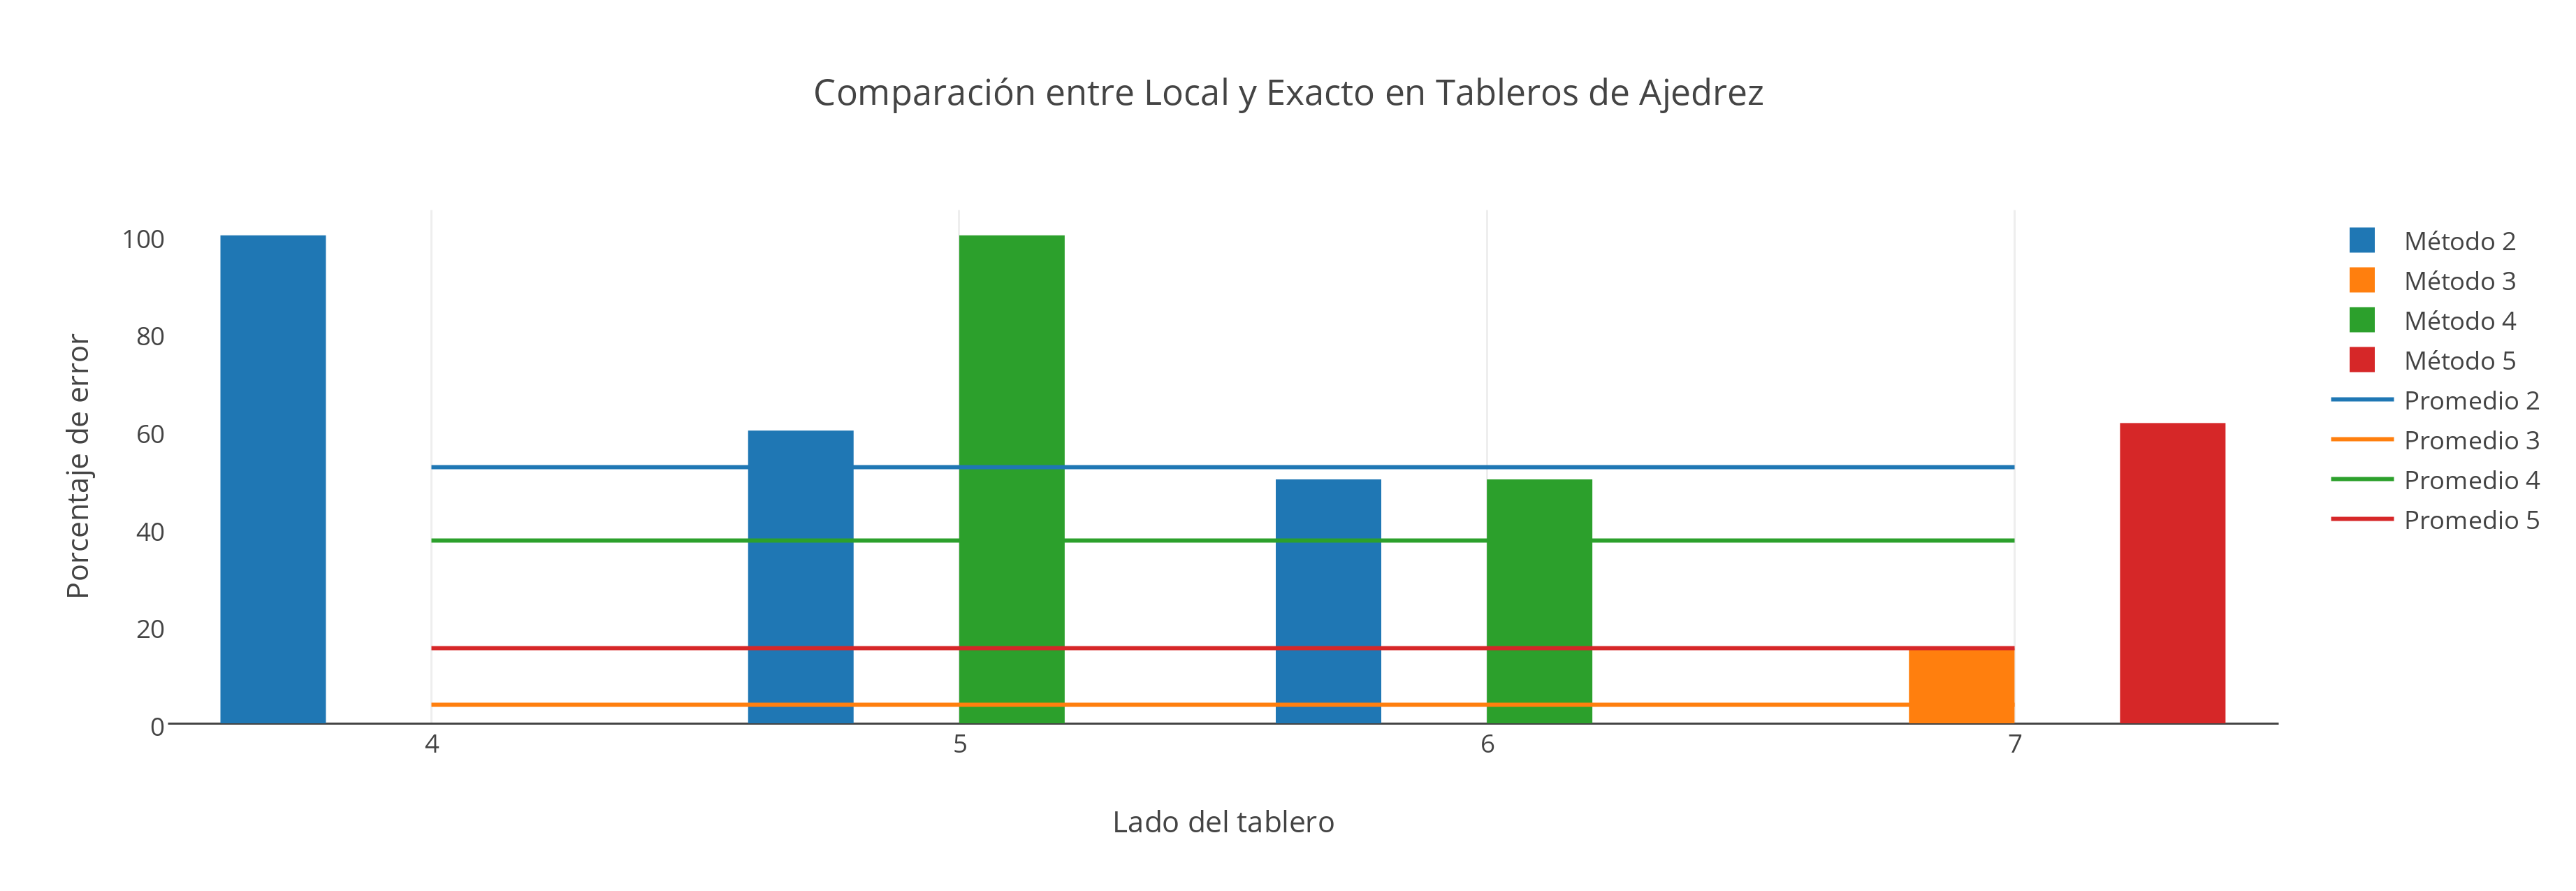
\includegraphics[scale=0.55]{imagenes/local/exacto/tableros.png}
% 	\caption{}
%	\label{10Nodos}
   \end{center}
 \end{figure} 
 
\newpage 
 
\subsubsection{Elecci\'on de versi\'on \'optima}

\newpage